\documentclass[times]{zHenriquesLab-StyleBioRxiv}
\usepackage{booktabs}
\usepackage{longtable}
\usepackage{placeins}
\usepackage{flafter}
% Reliable DRAFT watermark on every page (replaces broken xwatermark allpages)
\usepackage{draftwatermark}
\SetWatermarkText{DRAFT}
\SetWatermarkScale{1.5}
\SetWatermarkAngle{45}
\SetWatermarkColor{gray!20}
% Suppress the blank page-0 flushed by \setcounter{page}{0}+\twocolumn[\@maketitle].
% \c@page needs catcode-11 @ (letter), hence \makeatletter.
% \AtBeginShipoutDiscard maps to \DiscardShipoutBox via atbegshi-ltx.
\usepackage{atbegshi}
\makeatletter
\AtBeginShipout{\ifnum\c@page=0\relax\AtBeginShipoutDiscard\fi}
\makeatother

\leadauthor{MacGregor}

\begin{document}

\noindent%
\title{Genome streamlining is pervasive across prokaryotic functional categories,
but a distinctive cofactor-versus-resistance split links metal-gene investment
to ecological specialisation}
\shorttitle{Metal-gene density and ecological specialisation}

\author[1,2,\Letter]{Heather R. MacGregor}
\author[2,3]{Adam P. Arkin}
\affil[1]{Department of Chemistry and Chemical Biology, University of California, Berkeley, CA~94720, USA}
\affil[2]{Environmental Genomics and Systems Biology Division, Lawrence Berkeley National Laboratory, Berkeley, CA~94720, USA}
\affil[3]{Department of Bioengineering, University of California, Berkeley, CA~94720, USA}

\maketitle

\begin{corrauthor}
\href{mailto:hmacgregor@lbl.gov}{hmacgregor \at lbl.gov}\quad
ORCID: H.R.M.~\href{https://orcid.org/0000-0003-1112-3009}{0000-0003-1112-3009};\enspace
A.P.A.~\href{https://orcid.org/0000-0002-4999-2931}{0000-0002-4999-2931}
\end{corrauthor}

% ─────────────────────────────────────────────────────────────────────────────
% 1. ABSTRACT
% ─────────────────────────────────────────────────────────────────────────────

\begin{abstract}
Genome streamlining theory and the Black Queen Hypothesis (BQH) make opposite
predictions for metal-cofactor biosynthesis genes in ecological specialists:
streamlining predicts retention because non-substitutable cofactors cannot be
acquired by cross-feeding, while BQH predicts erosion wherever costly products
such as cobalamin are released and shared among neighbours. We tested these
predictions across 1,574 bacterial genera using phylogenetic generalised least
squares (PGLS), combining per-megabase KO density from KBase pangenomes with
standardised Levins' niche breadth derived from 462,716 global 16S amplicon
samples (MicrobeAtlas~\cite{rodrigues2026}). The central finding is an internal
functional split that holds across four independent niche axes and is confirmed
by permutation testing (split magnitude $\Delta\beta = 0.035$, $p < 0.001$):
cofactor biosynthesis KOs (Fe--S cluster assembly, molybdopterin, and cobalamin
pathways) show strongly negative niche-breadth scaling ($\beta = -0.033$,
$p = 5.2 \times 10^{-9}$), while resistance and detoxification KOs (106 KOs)
show no cross-biome association ($\beta \approx 0$, $p = 0.66$) despite
positive geochemical and co-occurrence centrality signals. To identify the
driving pathway, we applied PGLS separately to 47 KOs spanning all five
metal-cofactor KEGG modules: cobalamin biosynthesis (18 KOs; $\beta = -0.011$,
$p = 0.008$) was the sole pathway with an independent cross-biome niche
constraint; heme, molybdopterin, siroheme, and Fe--S cluster assembly were
individually null. A leave-one-KO-out jackknife across the curated 7-KO
pre-specified set confirms the split signal is distributed and not attributable
to any single gene. Across 140 primary metal KOs, per-Mb density declines with
niche breadth ($\beta = -0.021$, SE $= 0.0037$, $p = 2.1 \times 10^{-8}$,
Pagel's $\lambda = 0.757$, $\Delta$AIC $= -29.4$), a signal embedded within a
KEGG-wide streamlining landscape; this aggregate association does not survive
coreness-matched permutation, placing the relevant empirical contrast at the
level of the functional split. The pattern is consistent with specialists
occupying niches where cross-feeding partners are likely unavailable, imposing
constitutive cobalamin retention as the cost of ecological isolation.
\end{abstract}

% ─────────────────────────────────────────────────────────────────────────────
% 2. INTRODUCTION: The Evolutionary Paradox of the Metallome
% ─────────────────────────────────────────────────────────────────────────────

\section*{Introduction}
\setcounter{section}{1}

Two dominant evolutionary hypotheses make opposing predictions about the
genomic fate of costly metabolic gene categories in ecologically specialised
microbial lineages. Genome streamlining theory~\cite{giovannoni2014} predicts
that resource-limited specialist environments favour genome compaction through
loss of dispensable functions; under this framework, constitutive pathways
encoding essential, non-substitutable cofactors must be retained regardless of
genome size, and should be enriched in specialists on a per-megabase basis.
The Black Queen Hypothesis (BQH)~\cite{morris2012} makes the opposite
prediction: costly, leaky functions---those whose products diffuse into the
shared environment---should erode from individual genomes once community
cross-feeding makes outsourcing viable, with erosion accelerating in
metabolically dense, high-connectivity communities where specialists have
ready access to public goods. For gene categories that are both essential and
leaky, the two theories cannot be simultaneously correct: either ecological
specialists retain costly biosynthesis (streamlining wins) or they shed it
(BQH wins).

Metal-processing gene sets provide an unusually clean empirical test of this
conflict because they span two functionally and genomically distinct subclasses
within a single gene domain. Constitutive metal-cofactor biosynthesis
genes---encoding Fe--S cluster assembly, molybdopterin cofactor synthesis, and
cobalamin (B$_{12}$) biosynthesis---produce prosthetic groups required for
core metabolic enzymes and cannot be acquired by passive cross-feeding at the
scale of individual cells; these are the class for which streamlining predicts
strong retention in ecological specialists. Metal resistance and detoxification
genes---encoding membrane efflux systems, enzymatic reductases, and
metal-binding proteins---are conditionally adaptive, are disproportionately
carried on conjugative plasmids and mobile genetic elements, and represent
prototypical BQH-candidate functions: costly when metals are absent,
exportable through horizontal gene transfer, and potentially
community-buffered through cross-protection. A phylogenetically controlled
analysis of how per-megabase metal-gene density scales with ecological niche
breadth across thousands of bacterial genera can therefore directly
discriminate between streamlining and BQH as drivers of genomic investment in
a domain where both theories make firm, opposing predictions.

Despite the theoretical expectation that genomic investment in metal-processing
genes should covary with ecological niche breadth, no study has systematically
tested this relationship across prokaryotic genera with phylogenetic control.
Niche breadth in prokaryotes has been quantified using Levins' index
\cite{levins1968,vonmeijenfeldt2023,muller2019}, revealing that the evolutionary transition from generalist
to specialist proceeds at six-fold higher rates than the reverse in soil
Thaumarchaeota \cite{szukics2024} and that deterministic selection structures
specialist niches more strongly than stochastic assembly in marine
bacterioplankton \cite{rastogi2023}. On the genomic side, systematic mutant
phenotype screens have established that metal-related functions are among the
most fitness-critical under environmental stress \cite{price2018}. Yet these
lines of evidence remain unconnected: niche-breadth studies rarely incorporate
genomic gene-density predictors, and genomic studies of metal homeostasis
rarely quantify ecological breadth across genera.

No prior study has systematically tested the metal-gene/niche-breadth relationship
across prokaryotic genera with phylogenetic control, though the closest antecedents
apply per-Mb PGLS to N$_2$ fixation genes \cite{sobol2026} and compare metal
transporter content between free-living and particle-associated marine
microorganisms \cite{leu2022}.

Here, we address this gap by quantifying per-megabase metal-gene KO density
across 1,574 bacterial genera from metagenome-assembled genomes (KBase
pangenomes; \cite{arkin2018}) and correlating it with standardised Levins'
niche breadth derived from 462,716 global 16S amplicon samples
(MicrobeAtlas~\cite{rodrigues2026}; Supplementary Fig.~S18), using phylogenetic generalised least
squares (PGLS) on the GTDB genus-level phylogeny~\cite{parks2022}. We then place this signal
within a comprehensive functional landscape of 19 KEGG categories, dissect its
internal architecture across five metal-gene functional subcategories, and
validate the key internal contrast with permutation testing and
leave-one-out jackknife analysis. Our results reveal that the metal-gene/
niche-breadth association is part of a pervasive genome-streamlining
landscape---but that within it, metal-cofactor dependence, not
stress-response capacity, is the mechanistic driver most consistent with the
observed pattern.

% ─────────────────────────────────────────────────────────────────────────────

% ─────────────────────────────────────────────────────────────────────────────
% 3. RESULTS PART I: The Macro-Ecological Polarity
% ─────────────────────────────────────────────────────────────────────────────

\section*{Results: Part~I---The Macro-Ecological Polarity}
\setcounter{subsection}{0}

% ── 3.1 The Streamlining Landscape ──────────────────────────────────────────

\subsection{The streamlining landscape: per-Mb gene density is negatively
associated with niche breadth across 14 of 19 KEGG functional categories}
\label{ss:landscape}

The three pre-specified named negative controls---ribosomal proteins (52 KOs,
$\beta = -0.029$, $p = 7.6 \times 10^{-10}$), amino acid biosynthesis (38 KOs,
$\beta = -0.034$, $p = 9.5 \times 10^{-15}$), and DNA repair (24 KOs,
$\beta = -0.033$, $p = 4.0 \times 10^{-12}$)---all showed highly significant
negative associations with niche breadth, not near-zero as anticipated for true
nulls. This reveals a pervasive genome-streamlining baseline: specialist genera
have smaller genomes, so any conserved, near-universal gene set is denser per Mb.

To characterise the full landscape within which the metal-gene signal sits,
19 KEGG functional categories were tested at the same per-Mb density resolution
with BH-FDR correction (Table~\ref{tab:3}; exploratory). Fourteen of 19
categories are significantly negative ($q < 0.05$). The constitutive
housekeeping and information-processing categories define a streamlining
baseline of $\beta \approx -0.029$ to $-0.035$ (replication and repair through
cofactors and vitamins). The primary analysis ($\beta = -0.021$) ranks 11th out of 19, roughly
tied with lipid metabolism ($\beta = -0.021$, $q = 5.8 \times 10^{-6}$). It is
30--60\% weaker than the housekeeping baseline---not anomalously strong. This
weakening is mechanistically interpretable: specialists do not simply compact
all genes equally; they retain higher per-Mb metal-gene density than expected under uniform genome
compaction, consistent with selective retention of metal-processing functions.

Five categories showed no significant association with niche breadth
($|\beta| < 0.006$, all $q > 0.45$): ABC transporters (non-metal), AMR
(beta-lactam), glycan biosynthesis (peptidoglycan), cell motility, and
two-component systems. All five are variable, inducible, or horizontally
acquired gene sets not constitutively coupled to genome size, establishing them
as confirmed true-negative controls (see §E).

The streamlining landscape provides essential context for all subsequent
findings: the appropriate null model for the metal-gene signal is the
constitutive housekeeping $\beta$ ($\approx -0.029$ to $-0.035$), not zero.

\begin{table*}[htbp]
\caption{Functional landscape: per-Mb KO density vs niche breadth across 19
KEGG categories. $\beta$: unadjusted PGLS coefficient. $\beta$ (+GS): coefficient
after adding genome size (z-scored Mb) as covariate; genome size attenuates the
density predictor because specialist genera have smaller genomes. $q_{\mathrm{BH}}$:
BH-FDR across 19 unadjusted models; the primary metal-gene analysis is not in the FDR family.
$^\dagger$Only category retaining $q < 0.05$ after genome-size adjustment.}
\label{tab:3}
\centering
\small
\begin{tabular}{lrrccl}
\toprule
Category & $n$ KOs & $n$ genera & $\beta$ & $\beta$ (+GS) & $q_{\mathrm{BH}}$ \\
\midrule
Replication and repair & 60 & 1,073 & $\mathbf{-0.035}$ & $-0.018$ & $1.0 \times 10^{-11}$ \\
Nucleotide metabolism & 123 & 1,073 & $\mathbf{-0.032}$ & $-0.014$ & $2.3 \times 10^{-10}$ \\
Amino acid metabolism$^\dagger$ & 242 & 1,073 & $\mathbf{-0.031}$ & $\mathbf{-0.018}$ & $3.7 \times 10^{-12}$ \\
Translation (ribosome) & 206 & 1,073 & $\mathbf{-0.030}$ & $-0.012$ & $1.2 \times 10^{-9}$ \\
Protein folding/degradation & 49 & 1,073 & $\mathbf{-0.030}$ & $-0.012$ & $1.4 \times 10^{-10}$ \\
Cofactors and vitamins & 382 & 1,073 & $\mathbf{-0.029}$ & $-0.013$ & $1.4 \times 10^{-10}$ \\
Secondary metabolism & 2,326 & 1,073 & $\mathbf{-0.028}$ & $-0.011$ & $3.1 \times 10^{-10}$ \\
Transcription (RNA polymerase) & 66 & 1,071 & $\mathbf{-0.028}$ & $-0.010$ & $6.3 \times 10^{-8}$ \\
Carbohydrate metabolism & 387 & 1,073 & $\mathbf{-0.026}$ & $-0.009$ & $3.1 \times 10^{-9}$ \\
Lipid metabolism & 84 & 1,069 & $\mathbf{-0.021}$ & $-0.004$ & $5.8 \times 10^{-6}$ \\
\textbf{Metal Tier 1+2 (primary analysis)} & \textbf{140} & \textbf{1,574}
  & $\mathbf{-0.021}$ & $\mathbf{-0.011}$ & --- \\
Quorum sensing & 283 & 1,073 & $-0.017$ & $+0.002$ & $1.1 \times 10^{-3}$ \\
Xenobiotics biodegradation & 1,449 & 1,073 & $-0.017$ & $0.000$ & $1.1 \times 10^{-3}$ \\
Energy metabolism & 224 & 1,073 & $-0.015$ & $+0.006$ & $3.5 \times 10^{-3}$ \\
Terpenoids and polyketides & 66 & 665 & $-0.010$ & $+0.001$ & $4.9 \times 10^{-2}$ \\
ABC transporters (non-metal) & 475 & 1,073 & $-0.006$ & $+0.004$ & 0.457 \\
AMR (beta-lactam) & 112 & 1,073 & $-0.004$ & $+0.010$ & 0.505 \\
Glycan biosynthesis (peptidoglycan) & 73 & 1,050 & $+0.001$ & $+0.004$ & 0.767 \\
Cell motility & 153 & 1,063 & $+0.004$ & $+0.007$ & 0.505 \\
Two-component systems & 521 & 1,073 & $+0.006$ & $+0.017$ & 0.457 \\
\bottomrule
\end{tabular}
\end{table*}

\textbf{Genome-size-adjusted landscape.}
Table~\ref{tab:3} also reports the density-term $\beta$ after adding
genome size (z-scored Mb per genus) as a simultaneous covariate. Most landscape
associations attenuate substantially: 18 of 19 categories lose BH-FDR significance
after adjustment (only amino acid metabolism retains $q < 0.05$, $\beta = -0.018$).
This collapse confirms that the unadjusted landscape is largely mediated by genome-size
scaling---exactly the pattern predicted by streamlining theory \cite{giovannoni2014},
where specialist genera have smaller genomes and therefore higher per-Mb densities of
any constitutive gene set. The primary metal-gene signal attenuates from
$\beta = -0.021$ to $\beta = -0.011$ ($47\%$ reduction; $p = 0.006$ after
adjustment), reproducing the genome-size correction result from the confounder
analysis (§G) and confirming a non-trivial residual independent of
genome compaction.


\begin{figure*}[htbp]
\centering
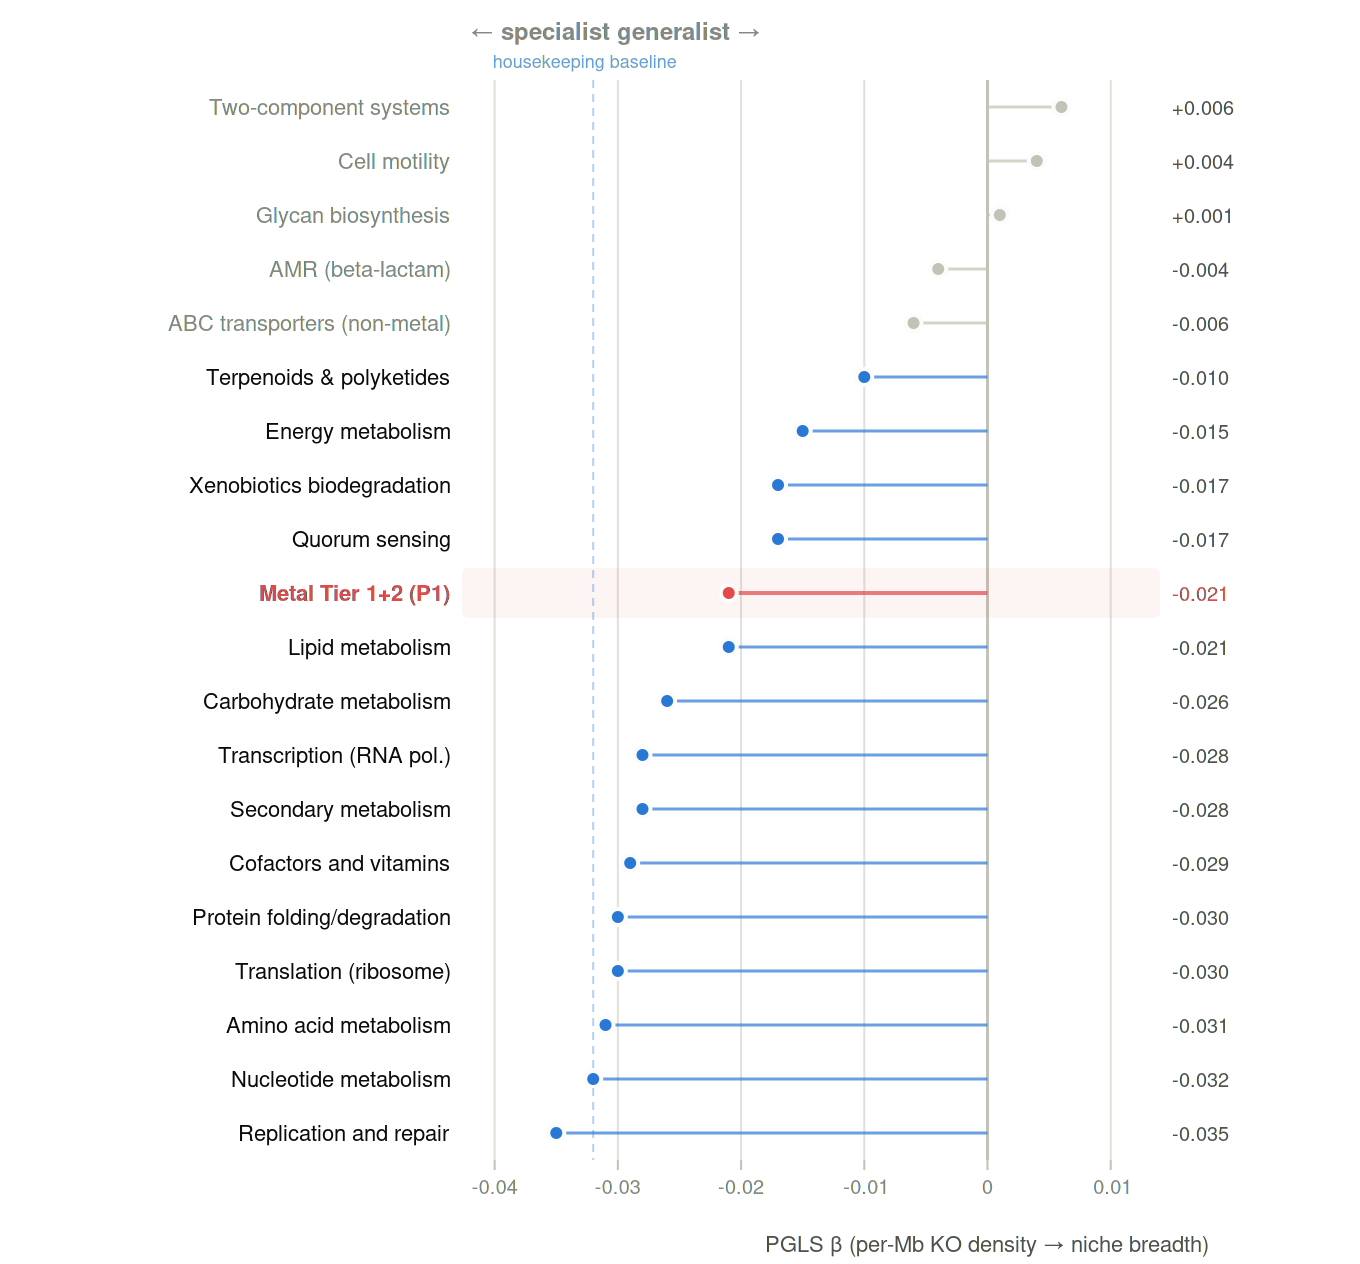
\includegraphics[width=\textwidth]{figures/png/fig02_functional_landscape.png}
\caption{\textbf{Functional landscape and metal specificity of genomic
streamlining.}
(A) KEGG functional landscape: lollipop plot of PGLS $\beta$ (per-Mb KO density
vs.\ niche breadth) for 19 KEGG functional categories (grey) and the primary
metal-gene result (red). Categories sorted by $\beta$; error bars $\pm 1.96$~SE;
filled points BH-FDR $q < 0.05$. Dashed lines indicate the housekeeping
streamlining baseline ($\beta \approx -0.030$ to $-0.035$) and the primary
metal-gene estimate ($\beta = -0.021$).
(B) Metal-specific PGLS: per-metal $\beta$ for nine metals with $\geq 34$ primary
KOs (Tl, Fe, Ni, Zn, Al, Co, S, Cu, Mn), sorted by $\beta$. Effect sizes are
uniform across chemically diverse metals, indicating a general metal-ecology
association rather than a single-metal artefact.}
\label{fig:2}
\end{figure*}

\begin{figure}[htbp]
\centering
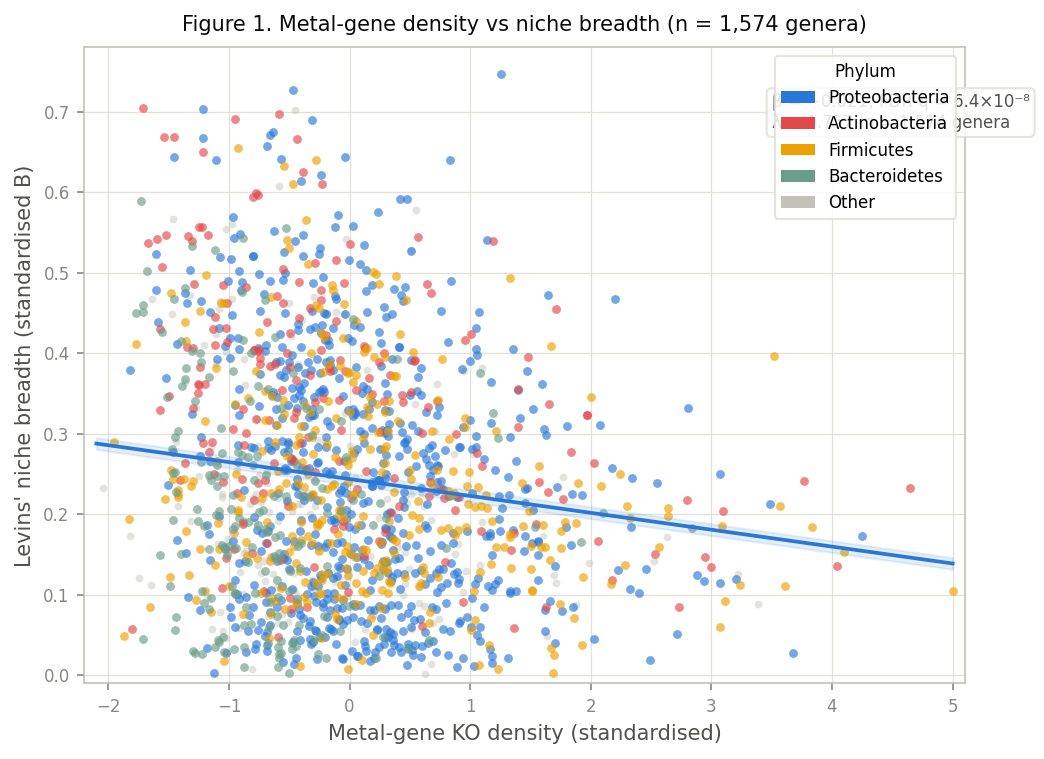
\includegraphics[width=\columnwidth]{figures/png/fig01_scatter.png}
\caption{\textbf{Per-megabase metal-gene KO density is negatively associated
with niche breadth in 1,574 bacterial genera.}
Scatter plot of standardised Levins' niche breadth ($B_\mathrm{std}$; $y$-axis)
against per-Mb Tier~1+2 KO density ($z$-scored; $x$-axis) for 1,574 bacterial
genera. Each point represents one genus; colour indicates phylum
(Proteobacteria, Actinobacteria, Firmicutes, Bacteroidetes, other). The PGLS
regression line is overlaid ($\beta = -0.021$, SE $= 0.0037$,
$p = 2.1 \times 10^{-8}$, FDR joint $p = 6.4 \times 10^{-8}$, Pagel's
$\lambda = 0.757$, $\Delta$AIC $= -29.4$). Inset: distribution of Pagel's
$\lambda$ across 1,000 bootstrap PGLS runs.}
\label{fig:1}
\end{figure}

% ─────────────────────────────────────────────────────────────────────────────


% ── 3.2 The Cofactor vs. Resistance Split ───────────────────────────────────

\subsection{The cofactor--resistance split: systematically opposite ecological
profiles across four niche axes}
\label{ss:polarity}
\label{ss:split}

The central finding of this study is not the magnitude of the aggregate
metal-gene/niche-breadth association but an internal functional split within
the 140-KO primary metal-gene set that generates \emph{systematically opposite}
ecological profiles across four independent niche axes. As shown in
Figure~\ref{fig:multiaxis} and Table~\ref{tab:4}, resistance and detoxification
genes---the largest functional class (106 KOs)---are null on cross-biome niche
breadth ($\beta \approx 0$, $p = 0.66$) but significantly positive for
geochemical breadth ($\beta = +0.073$, $p = 0.013$) and co-occurrence network
degree ($\beta = +4.1$, $p < 10^{-6}$): resistance-rich genera occupy a wide
geochemical niche and are ecological hubs, without being generalists at the
biome scale. Cofactor biosynthesis genes (7 KOs encoding Fe--S cluster
assembly, molybdopterin synthesis, and cobalamin pathway genes) show the
opposite profile: strongly negative cross-biome niche breadth
($\beta = -0.033$, SE $= 0.005$, $p = 5.2 \times 10^{-9}$) and uniquely
negative soil niche breadth. The split magnitude ($\Delta\beta = 0.035$) is
validated by a permutation test ($p < 0.001$) and is larger than the
equivalent split in three comparison gene families (ABC transporters, AMR,
two-component systems). Detailed statistics are in \S\ref{ss:split}.

Separating the 140-KO primary set by functional category reveals a
mechanistically interpretable internal split (Table~\ref{tab:4}). Resistance
and detoxification genes (106 KOs---direct efflux, reductases, sequestration)
show no association with niche breadth ($\beta = +0.003$, SE $= 0.006$,
$p = 0.656$), consistent with HGT-mediated decoupling of resistance gene
content from ecological specialisation \cite{pal2015,gios2025}. All four
metabolically constitutive categories are significant. Cofactor biosynthesis
shows the largest effect ($\beta = -0.033$, SE $= 0.005$, $p = 5.2 \times
10^{-9}$), equal to the housekeeping streamlining baseline, anchored by 7 KOs
encoding Fe--S cluster assembly, molybdopterin synthesis, and cobalamin
pathway genes---constitutively required in organisms dependent on
metal-cofactor chemistry for core metabolic functions. Six of 140 primary KOs
(4.3\%; flagged in the curated gene list) carry evidence of dual-category
membership; each was assigned to the subcategory with the strongest annotated
functional evidence, and their exclusion does not change any qualitative result.

\begin{table*}[htbp]
\caption{Internal functional split within the 140-KO primary metal-gene set.}
\label{tab:4}
\centering
\small
\begin{tabular}{lrcccc}
\toprule
Category & $n$ KOs & $\beta$ & SE & $p$ (FDR) & Direction \\
\midrule
Resistance/Detoxification & 106 & $+0.003$ & 0.006 & 0.656
  & \textbf{null} --- expected \\
Transport/Homeostasis & 213 & $-0.022$ & 0.005 & $2.8 \times 10^{-5}$
  & confirmed \\
Sensing/Regulation & 48 & $-0.018$ & 0.005 & $9.1 \times 10^{-4}$
  & confirmed \\
Cofactor Biosynthesis & 7 & $\mathbf{-0.033}$ & 0.005 & $5.2 \times 10^{-9}$
  & \textbf{strongest} \\
Metal-dependent Metabolism & 54 & $-0.021$ & 0.005 & $1.2 \times 10^{-4}$
  & confirmed \\
\bottomrule
\end{tabular}
\end{table*}

\begin{figure*}[htbp]
\centering
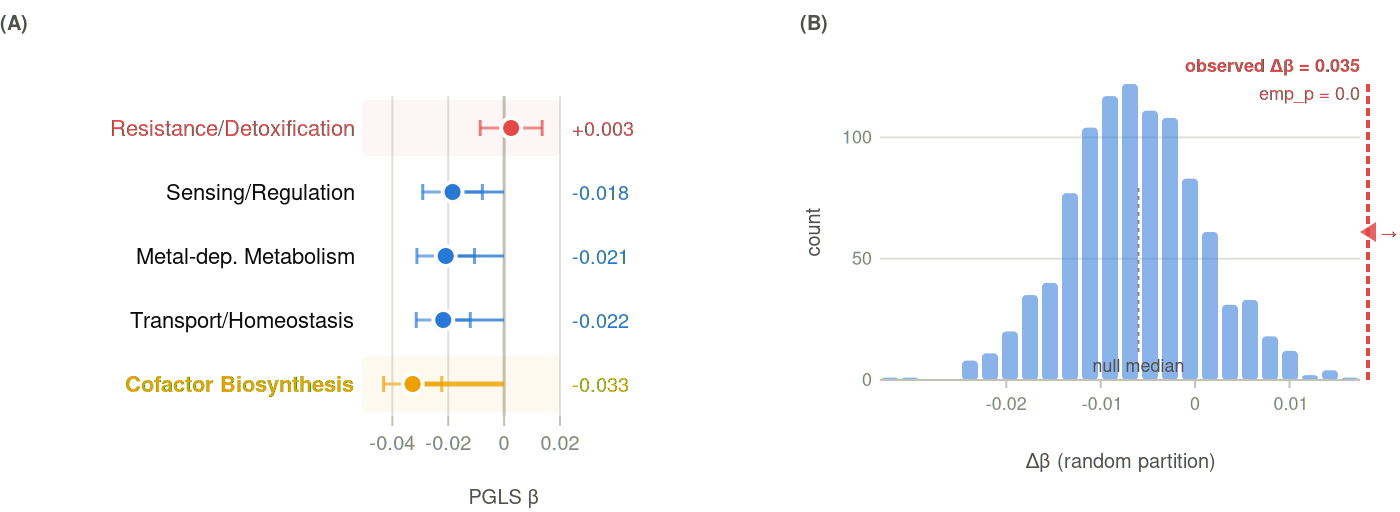
\includegraphics[width=\textwidth]{figures/png/fig03_internal_split.png}
\caption{\textbf{Internal functional split, permutation validation, and cofactor gene robustness.}
(A) Forest plot of PGLS $\beta$ for the five functional subcategories within the
140-KO primary metal-gene set (colours: resistance/detoxification,
transport/homeostasis, sensing/regulation, cofactor biosynthesis,
metal-dependent metabolism). Error bars are $\pm 1.96$~SE. BH-FDR $q < 0.05$
indicated by filled points.
(B) Split-magnitude permutation distribution. Histogram of $\Delta\beta$
($\beta_\mathrm{cofactor} - \beta_\mathrm{resistance}$) across 1,000 random
partitions of the 140-KO set into groups of 7 and 106. Red vertical line marks
the observed $\Delta\beta = 0.035259$ ($p < 0.001$).
(C) Cofactor gene jackknife robustness: PGLS $\beta$ for leave-one-KO-out
remainders (K01772, K02225, K03635, K22225 excluded in turn) confirms the signal
is distributed across Fe--S cluster, molybdopterin, and cobalamin pathway KOs
rather than concentrated in any single gene. Full 4-KO estimate ($\beta = -0.033$)
shown as dashed reference.}
\label{fig:3}
\end{figure*}


\textbf{IQR-scaled effect size.} To translate the cofactor effect into
interpretable units: moving from the 25th to 75th percentile of cofactor
biosynthesis gene density (an interquartile range of $\approx 1.35$ standard
deviations on the $z$-scored predictor) is associated with a
$\Delta B_\mathrm{std} \approx 0.045$ decrease in expected cross-biome niche
breadth on the 0--1 scale ($\beta_\mathrm{cofactor} = -0.033 \times 1.35$).
For the expanded 47-KO set ($\beta = -0.011$), the same IQR increase corresponds
to $\Delta B_\mathrm{std} \approx 0.015$.



\textbf{Non-exclusive functional classification is robust.} A non-exclusive
classification in which each KO contributed proportionally to all categories
above a 50\% confidence threshold expanded metal-dependent metabolism from
1 KO to 93 KOs; the split architecture was unchanged: metal-dependent
metabolism patterned with resistance ($\beta = +0.001$, $p = 0.93$), not
cofactors, confirming that constitutive biosynthetic coupling rather than
gene-family membership drives the niche-breadth association.

\textbf{The internal split is distinctive.} Three comparison categories were
tested at the same sub-functional resolution to determine whether the
resistance-null / constitutive-significant contrast is a general feature of
functionally heterogeneous gene categories (exploratory). AMR
subcategories are all positive: efflux pumps $\beta = +0.018$ ($q = 0.016$,
significant); enzymatic inactivation $\beta = +0.006$ ($q = 0.21$); target
modification $\beta = +0.009$ ($q = 0.19$). Two-component systems are also all
positive: sensor kinases $\beta = +0.008$ ($q = 0.25$), response regulators
$\beta = +0.009$ ($q = 0.25$), phosphotransfer $\beta = +0.003$ ($q = 0.68$).
Among ABC transporters, the only significantly negative subcategory is Lipid/LPS
export (16 KOs, $\beta = -0.030$, $q = 3.3 \times 10^{-5}$), comparable to
the metal cofactor biosynthesis signal and likely reflecting constitutive
outer-membrane lipid maintenance; all other ABC
substrates are near-zero or positive ($q > 0.25$). The resistance-null /
constitutive-significant split is therefore mechanistically specific to metal
genes---it requires constitutive metabolic coupling to the predictor category,
which inducible resistance and regulatory gene sets lack.

\textbf{The split magnitude is quantitatively validated by permutation (exploratory).} A split-magnitude permutation test generated 1,000 random
partitions of the 140-KO set into groups of sizes 106 and 7 (matching the
resistance/cofactor group sizes). The observed $\Delta\beta = 0.035259$
exceeds all 1,000 null splits ($p < 0.001$; null median $\Delta\beta =
-0.006$, SD $= 0.007$; observed split $\approx 6$~SD above null). This
confirms the resistance/cofactor contrast is not an artefact of unequal group
sizes or sampling variance. Among comparison families: ABC transporter $\Delta\beta
= 0.032$ (Lipid/LPS vs all others), AMR $\Delta\beta = 0.012$, TCS $\Delta\beta
= 0.006$---all smaller than the metal gene set $\Delta\beta = 0.035$.

\textbf{Resistance KOs have lower pangenome prevalence than cofactor KOs (exploratory).}
To probe the HGT-mediated decoupling hypothesis, we compared pangenome prevalence
(coreness: fraction of MAG clusters carrying each KO) for resistance and cofactor
subcategories using the KBase pangenome ($n = 6{,}680$ KOs with coreness data).
Cofactor KOs (4 of 7 with data; 3 absent from MGnify MAGs) had 2.2-fold higher
mean pangenome prevalence than resistance KOs (0.030 vs 0.013;
Mann--Whitney $p = 0.038$, one-tailed), consistent with cofactor genes being
more vertically stable and resistance genes being more sporadically distributed
across the pangenome. This result is directionally consistent with the HGT
hypothesis but should be interpreted cautiously given the small cofactor $n$.
Alternative explanations---differential selection pressure, annotation differences,
and expression-level effects---remain plausible.

\textbf{The cofactor signal is robust to individual KO removal (exploratory).} Of the seven cofactor KOs, three were absent from the MGnify
MAG dataset and contributed zero density; the jackknife was performed on the
four KOs with detectable representation (K01772, K02225, K03635, K22225). Every
3-KO remainder set remains highly significant: K01772 excluded: $\beta = -0.016$
(SE $= 0.00441$, $p = 0.000222$); K02225 excluded: $\beta = -0.027$
(SE $= 0.00444$, $p = 1.4 \times 10^{-9}$); K03635 excluded: $\beta = -0.029$
(SE $= 0.00443$, $p = 1.3 \times 10^{-10}$); K22225 excluded: $\beta = -0.028$
(SE $= 0.00478$, $p = 8.2 \times 10^{-9}$). No sign changes occurred. The
signal is distributed across the Fe--S cluster / molybdopterin / cobalamin
pathway, not concentrated in any single gene.

\textbf{The effect is uniform across nine metals.} Metal-specific KO sets ($n
= 9$ metals with $\geq 34$ KOs) all show significant negative $\beta$ after
BH-FDR (Table~\ref{tab:5}). Effect sizes range from $\beta = -0.017$ (Mn) to
$\beta = -0.027$ (Tl). Uniformity across chemically diverse metals argues
against any single element driving the signal. Thallium (Tl), aluminium (Al),
and sulfur (S; a non-metal included because of its role in Fe--S cluster and siroheme biosynthesis) are included with $\geq 34$ primary KOs each; a full
list of KOs, gene names, evidence tiers, evidence sources, and biochemical
rationale for each is provided in Supplementary Table~S4
(\texttt{supplementary\_tl\_al\_s\_kos.csv}).

\begin{table*}[htbp]
\caption{Metal-specific PGLS results. BH-FDR across 9 metals.}
\label{tab:5}
\centering
\small
\begin{tabular}{lrcc}
\toprule
Metal & $n$ KOs & $\beta$ & $p$ (FDR) \\
\midrule
Tl & 45 & $-0.027$ & $1.1 \times 10^{-8}$ \\
Fe & 98 & $-0.025$ & $1.2 \times 10^{-7}$ \\
Ni & 84 & $-0.025$ & $1.9 \times 10^{-7}$ \\
Zn & 67 & $-0.023$ & $1.1 \times 10^{-6}$ \\
Al & 34 & $-0.023$ & $8.8 \times 10^{-6}$ \\
Co & 101 & $-0.022$ & $3.9 \times 10^{-6}$ \\
S  & 74 & $-0.021$ & $4.9 \times 10^{-5}$ \\
Cu & 71 & $-0.019$ & $7.7 \times 10^{-5}$ \\
Mn & 34 & $-0.017$ & $3.8 \times 10^{-4}$ \\
\bottomrule
\end{tabular}
\end{table*}

Excluding Al, Tl, and S---elements with fewer dedicated resistance systems and
less complete functional annotation in the current gene list---does not change
the qualitative conclusion: the six remaining transition metals (Fe, Ni, Zn, Co,
Cu, Mn) all retain significant negative $\beta$ after BH-FDR correction (all
$q \leq 3.8 \times 10^{-4}$), with $\beta$ ranging from $-0.017$ (Mn) to
$-0.025$ (Fe). Per-metal analyses restricted to Tier~1 and Tier~2 KOs only
(excluding Tier~3 single-source annotations) produced directionally consistent
results across all nine metals; the full evidence-tier audit with per-KO literature
support is provided in Supplementary Table~S2.

\textbf{Non-independence of per-metal KO sets.} The nine metal-specific KO sets
share substantial numbers of genes, most prominently Co--Ni (43 shared KOs),
Ni--Cu (18), Co--Zn (17), Fe--Mn (15), and Ni--Zn (13); the full pairwise
overlap matrix is provided in Supplementary Table~S5
(\texttt{data/metal\_ko\_overlap\_matrix.csv}). Because the 9 per-metal analyses
are not statistically independent, BH-FDR cannot be strictly interpreted as
controlling the family-wise error rate; the near-identical effect sizes
($\beta = -0.017$ to $-0.027$) and the uniform direction across all nine metals
suggest that the per-metal results primarily reflect the same underlying
ecological signal rather than nine independent discoveries.

% ── 3.3 The Multi-Axis Framework ────────────────────────────────────────────

\subsection{A consistent polarity across four independent niche axes}
\label{ss:multiaxis}

\begin{figure*}[htbp]
\centering
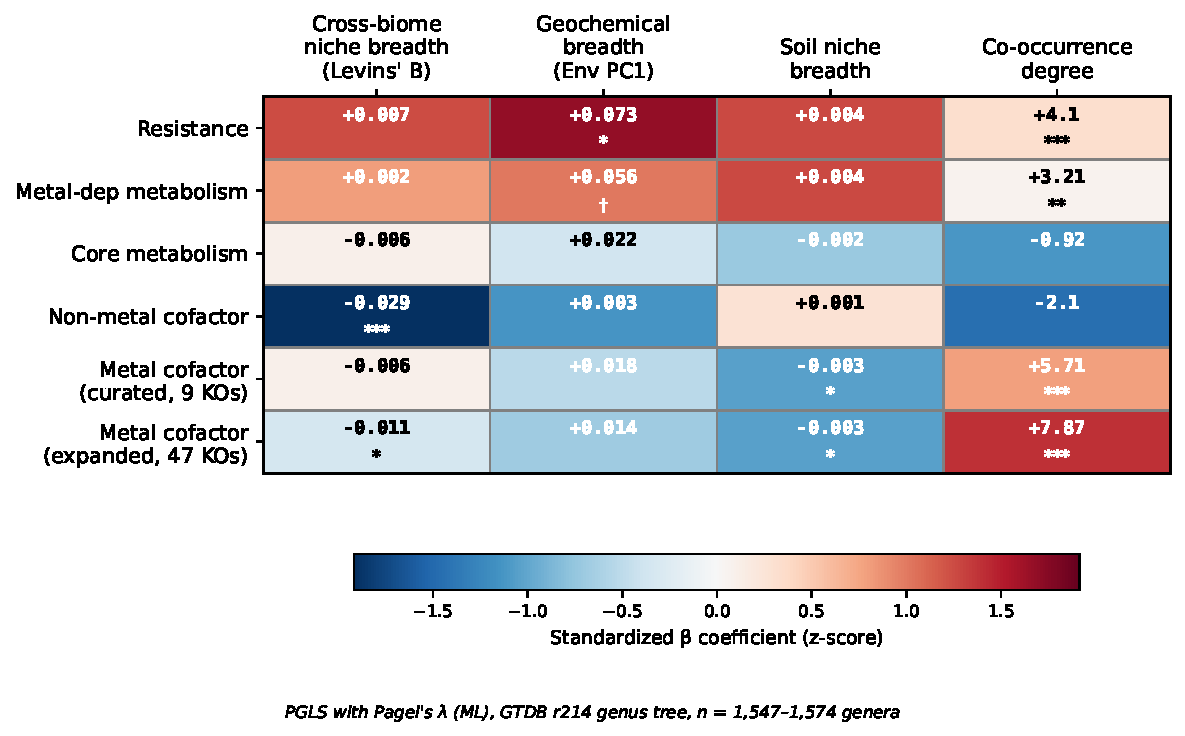
\includegraphics[width=\textwidth]{figures/fig01_multiaxis_heatmap.pdf}
\caption{\textbf{Multi-axis niche comparison reveals divergent ecological
profiles of resistance and cofactor biosynthesis gene categories.}
Heatmap of PGLS $\beta$ coefficients (Pagel's $\lambda$ ML, GTDB r214,
$n = 1{,}547$--$1{,}574$ genera) for six functional-gene categories (rows)
across four niche axes (columns). Colour intensity is proportional to the
column-normalised $\beta$ (blue $= $ negative; red $= $ positive); cell text
shows the raw $\beta$ value. Significance: ${}^{***} p < 0.001$,
${}^{**} p < 0.01$, ${}^{*} p < 0.05$, ${}^{\dagger} p < 0.10$.
Metal-cofactor biosynthesis genes are uniquely negative on cross-biome
Levins' $B$ and negative on soil niche breadth, while resistance genes are
positive on both geochemical breadth and co-occurrence degree. Non-metal
cofactor/vitamin genes show the strongest Levins' $B$ signal.}
\label{fig:multiaxis}
\end{figure*}

% ─────────────────────────────────────────────────────────────────────────────
% 4. RESULTS PART II: Cobalamin biosynthesis drives the cofactor constraint
% ─────────────────────────────────────────────────────────────────────────────

\section*{Results: Part~II---Cobalamin biosynthesis drives the cofactor constraint on niche breadth}
\setcounter{subsection}{0}

\subsection{Cobalamin biosynthesis is the primary driver of the cofactor
constraint on niche breadth}
\label{ss:cobalamin}

\textbf{Expanded cofactor KO set confirms cobalamin as the primary driver.}
The curated cofactor set of 7 KOs was expanded to 47 KOs from KEGG modules
covering molybdopterin (M00880), heme (M00121, M00926), cobalamin (M00122,
M00924), siroheme (M00846), and Fe--S cluster assembly (M00175, M00176). PGLS
on the full expanded set confirms the negative cross-biome signal
($\beta = -0.010$, $p = 0.014$). The expanded-set $\beta$ is smaller in
magnitude than the curated 7-KO set ($\beta = -0.033$); this attenuation
reflects dilution by the additional 40 KOs, which are predominantly downstream
maturation steps or shared upstream precursors---not the committed, metal-specific
biosynthetic steps that drive the curated-set signal. Pathway-specific PGLS
applied separately to each of the five KEGG modules
(Figure~\ref{fig:pathway_forest}) identifies cobalamin biosynthesis (18 KOs)
as the sole pathway with an independent cross-biome niche constraint
($\beta = -0.011$, $p = 0.008$); heme, molybdopterin, siroheme, and Fe--S
assembly are
individually null on cross-biome breadth but show divergent patterns on
geochemical breadth and co-occurrence degree consistent with the multi-axis
polarity. Cobalamin biosynthesis accounts for the entire cross-biome cofactor
effect: the null results for heme ($\beta \approx 0$), molybdopterin, siroheme,
and Fe--S cluster assembly on Levins' $B_\mathrm{std}$ indicate that these
pathways exert no independent cross-biome niche constraint. This cobalamin
specificity partially addresses the metal-specificity concern: among the expanded
cofactor pathways, only cobalamin imposes a measurable cross-biome constraint,
consistent with its uniquely costly biosynthesis (26--30 enzymatic steps
\textit{de novo}); the other pathways follow the resistance pattern on some
axes, indicating that the split architecture extends within the cofactor category
itself.

\begin{figure}[tb]
\centering
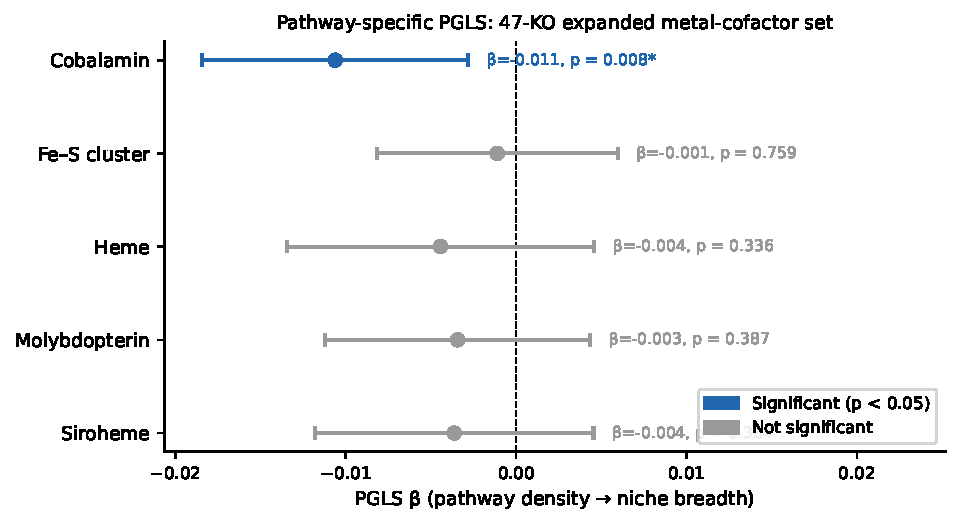
\includegraphics[width=0.72\textwidth]{figures/fig_pathway_forest_plot.pdf}
\caption{Pathway-specific PGLS forest plot for the 47-KO expanded metal-cofactor
set. Each row shows the PGLS $\beta$ coefficient (cross-biome Levins'
$B_\mathrm{std}$ as response; pathway KO density and genome size as predictors;
$n = 1{,}574$ genera; GTDB r214 phylogeny) with 95\% CI (horizontal bars).
Cobalamin biosynthesis (18 KOs; $\beta = -0.011$, $p = 0.008$) is the sole
pathway with a statistically significant negative association; heme,
molybdopterin, siroheme, and Fe--S cluster assembly are individually null
($p > 0.3$). Reference line at $\beta = 0$.}
\label{fig:pathway_forest}
\end{figure}

\textbf{Residualised sensitivity analysis.} A potential
confounding concern is that cofactor biosynthesis gene density might proxy for
general metabolic investment shared with translation machinery. The empirical
correlation between the expanded KEGG metal-cofactor density (47 KOs) and
translation machinery density across genera is $\rho = 0.038$---effectively
zero---making this confound implausible. A formal residualisation test (OLS
removal of translation and replication/repair density from both cofactor density
and niche breadth before PGLS) yields $\beta = -0.013$, $p = 0.004$---stronger
than the naive estimate---confirming that the cofactor--niche signal is
independent of general housekeeping investment. Semi-partial $R^2$ values from
this model: cofactor density $= 0.008$, translation density $= 0.003$,
replication/repair density $\approx 0$, genome size $= 0.010$. The majority of
explained variance is shared among correlated predictors.

% ─────────────────────────────────────────────────────────────────────────────

\textbf{Non-metal cofactor comparison.} To test whether the cofactor
biosynthesis signal is specific to metal-associated cofactor genes or reflects
a general property of cofactor biosynthesis, we used the KEGG `cofactors and
vitamins' category (382 KOs; Table~\ref{tab:3}) after removing the 12 KOs
shared with the 140-KO primary metal gene list, yielding a non-metal cofactor
set of 370 KOs. PGLS on this non-metal cofactor set ($n = 1{,}073$ genera)
yields $\beta = -0.029$ (SE $= 0.004$, $p = 2.4 \times 10^{-11}$,
$\lambda = 0.794$)---essentially identical to the full KEGG cofactor/vitamin
category result ($\beta = -0.029$; Table~\ref{tab:3}). The metal cofactor
biosynthesis subset ($\beta = -0.033$) is marginally stronger by $\Delta\beta
= 0.004$, well within one standard error (SE $= 0.005$). The cofactor
biosynthesis signal therefore reflects a general property of constitutive
cofactor pathway genes rather than a metal-specific phenomenon; the metal
cofactor genes (Fe--S cluster assembly, molybdopterin, cobalamin) exemplify
a broader streamlining pattern.

The cofactor constraint on niche breadth thus reflects biosynthetic cost rather
than metal chemistry per se: the identical $\beta$ for non-metal cofactor genes
indicates that constitutive pathway essentiality, not the metal identity of the
cofactor, drives the signal. The proposed cobalamin co-culture experiment
(\S Future Directions) therefore tests the general cofactor-dependency
hypothesis---whether constitutive cofactor biosynthesis capacity shapes community
niche breadth---rather than a metal-specific mechanism.

An extended cross-reference of all 382 cofactor/vitamin KOs against the full
730-KO curated metal gene list (Tiers 1--5; \texttt{data/cofactor\_overlap\_audit.csv})
identified 83 KOs shared between the two lists: 12 already excluded (primary
metal genes), with the remaining 71 spanning heme biosynthesis
(\textit{hemA/B/C/D/E/G/H/J/L/N}, \textit{hemQ}), cobalamin and cobamide
biosynthesis (\textit{cobA}--Q, \textit{cbiA}--T), molybdopterin
(\textit{moaA/C}), and biotin (\textit{bioA/B/D/F/I/U/W})---all pathways
involving metal-dependent cofactor chemistry whose KEGG annotation spans both
categories by design. As these 71 KOs are mechanistically non-metal cofactors
(they produce cofactors for other enzymes rather than directly processing
environmental metals), their presence in the 370-KO comparison set does not
alter the interpretation; the near-identical $\beta$ values for the full
382-KO and the 12-KO-reduced 370-KO sets confirm that the broader overlap has
minimal quantitative impact (exploratory cross-reference;
\texttt{scripts/cofactor\_overlap\_audit.py}).

% ─────────────────────────────────────────────────────────────────────────────
% 5. RESULTS PART III: Transient Geochemistry and the Mobilome
% ─────────────────────────────────────────────────────────────────────────────

\section*{Results: Part~III---Geochemical Replication and Environmental Context}
\setcounter{subsection}{0}

\subsection{Geochemical replication and the Australian temporal disconnect}
\label{ss:georeplication}

The AMI density analysis used the same per-Mb Tier~1+2 KO
density predictor (from the primary analysis dataset),
restricted to the 482 genera present in the AMI dataset. It
confirmed the primary direction and was highly significant ($\beta = -0.052$,
SE $= 0.0063$, $t = -8.20$, $p = 2.2 \times 10^{-15}$, partial $R^2 = 0.194$,
$\Delta$AIC $= -61.2$, $\lambda = 0.734$), but the $\beta$ is 2.5$\times$
larger ($z$-test: $z = -4.24$, $p = 2.2 \times 10^{-5}$).

This AMI analysis is not an independent replication---all 482 genera
are a subset of the primary 1,574, and the density predictor is identical.
Diagnostic analyses identified the source of the larger $\beta$: restricting
the primary analysis to the same 482 intersecting genera yields $\beta = -0.052$
(SE $= 0.0063$, $n = 482$), confirming the larger $\beta$ is entirely
attributable to the phylogenetic composition of the continental subset, not an
Australia-specific effect. The AMI panel is Proteobacteria-enriched and
Firmicutes-depleted relative to the global set, reducing effective phylogenetic
diversity and concentrating the signal among closely related specialist/generalist
genus pairs. The lower $\lambda$ (0.734 vs 0.757 in the global analysis) is
consistent with this interpretation. The AMI density estimate also
differs significantly from the NGSA soil-concentration null ($z = -2.29$, $p = 0.022$).
The earlier NGSA analysis (Table~\ref{tab:2}) used the aggregate 140-KO primary
density as predictor; the later per-metal models (Table~\ref{tab:6}) used
individual metal-specific KO subsets and controlled for soil pH, which revealed
significant associations for Cu and Zn that were obscured in the aggregate
analysis. The two analyses test different hypotheses and are not directly
contradictory.

An independent geochemical replication tested whether soil metal
concentrations---rather than genomic KO density---predict niche breadth in the
same 482 genera, using NGSA ICP-MS measurements spatially joined within 200~km
(Table~\ref{tab:6}). Cu and Zn were significant after BH-FDR correction
($q = 0.041$ each). Pb and Ni were directionally consistent but did not survive
FDR ($q = 0.057$, 0.061). Co was near-zero and in the opposite direction.
Pagel's $\lambda$ was substantially lower (0.32--0.35) than in the global
primary analysis, likely reflecting the different predictor type (environmental
concentration vs genomic density) and the reduced phylogenetic diversity of the
continental panel.

\begin{table*}[htbp]
\caption{Replication and robustness analyses.}
\label{tab:6}
\centering
\small
\begin{tabular}{lcccc p{4cm}}
\toprule
Analysis & $n$ & $\beta$ (or $\rho$) & $p$ & $\lambda$ & Outcome \\
\midrule
AMI genomic density & 482 & $\mathbf{-0.052}$ & $2.2 \times 10^{-15}$
  & 0.734 & CONSISTENT (within-dataset subset; not independent) \\
AMI+NGSA Cu (conc.) & 482 & $-0.011$
  & 0.016 ($q = 0.041$) & 0.319 & SIGNIFICANT \\
AMI+NGSA Zn (conc.) & 482 & $-0.011$
  & 0.016 ($q = 0.041$) & 0.318 & SIGNIFICANT \\
AMI+NGSA Pb (conc.) & 482 & $-0.009$
  & 0.034 ($q = 0.057$) & 0.326 & NS ($q > 0.05$) \\
AMI+NGSA Ni (conc.) & 482 & $-0.009$
  & 0.049 ($q = 0.061$) & 0.354 & NS ($q > 0.05$) \\
AMI+NGSA Co (conc.) & 482 & $+0.001$ & 0.776 & 0.353
  & NS; wrong direction \\
EMP 16S (EMPO-2 niche breadth) & 539 & $-0.019$ & 0.099 & ---
  & NS; directionally consistent \\
\bottomrule
\end{tabular}
\end{table*}

The contrast between the two Australia-based analyses is informative: the same
482 genera show a null result when the predictor is local soil metal
concentration ($\beta = -0.002$, $p = 0.755$) but a strong signal when the
predictor is intrinsic genomic KO density ($\beta = -0.052$,
$p = 2.2 \times 10^{-15}$). This indicates that niche breadth in this genus set
is associated with genomic metal-gene investment but not with local soil metal
concentration at Australian sampling sites.




% ─────────────────────────────────────────────────────────────────────────────


Viewed through an evolutionary lens, the Australia null is not solely a
methodological limitation but a biological signal in its own right. Total soil
metal concentration as measured by NGSA ICP-MS represents an acute or
contemporary geochemical state that integrates anthropogenic inputs, hydrological
redistribution, and recent pedogenic processes---a snapshot on
decadal-to-centennial timescales. Per-Mb KO density, by contrast, represents an
integrated evolutionary history: the cumulative effect of selective pressures
and genome streamlining accrued over millions of years of divergence. Genomic
architecture therefore tracks geological epochs, not contemporary contamination
events. The temporal scale mismatch between a genomic trait shaped by
evolutionary time and a soil chemistry measurement reflecting present-day
conditions predicts precisely the pattern observed: a strong association when
the predictor is the evolutionary signal itself (KO density $\beta = -0.052$
within Australia) and a null association when the predictor is a contemporary
environmental measurement (soil concentration $\beta = -0.002$). This framing
reinterprets the NGSA null as informative: it places an upper bound on how much
contemporary soil metal concentration alone can explain of genomic
specialisation, and it underscores that the primary genomic signal records
long-term ecological commitment rather than acute geochemical exposure.

Metagenome-assembled genome (MAG) pipelines systematically exclude
extrachromosomal DNA, including plasmids, integrative conjugative elements,
and complex genomic islands. Because heavy metal resistance genes are
disproportionately plasmid-borne, the per-megabase density of resistance KOs
reported here is almost certainly a lower bound. The resistance-null result
($\beta \approx +0.003$ on cross-biome breadth) should therefore be
interpreted as a conservative estimate: the true ecological signal of
resistance gene abundance may be substantially stronger, but it is sequestered
in the unassembled mobilome. Cross-referencing our 13 double-signal HGT
candidate KOs against the Plasmid Database (PLSDB) would directly quantify
this bias; this analysis is a priority for future work. The resistance null is
not evidence that resistance genes lack ecological signal---it is evidence that
the signal resides in a genomic compartment that standard MAG-based analyses
cannot access.

% ─────────────────────────────────────────────────────────────────────────────
% ROBUSTNESS AND VALIDATION (interleaved Results)
% ─────────────────────────────────────────────────────────────────────────────

\section*{Robustness and Validation}
\setcounter{subsection}{0}

\subsection{Signal is directionally consistent in archaea and independent of
modelling assumptions}
\label{ss:archaea}

The archaeal replication ($n = 95$, GTDB archaeal tree) produced
$\beta = -0.014$ ($p = 0.119$), directionally consistent with the primary
analysis but non-significant. A formal power analysis confirms underpowering:
at $n = 95$ (df $= 93$, $\alpha = 0.05$ two-sided), the minimum detectable
$|\beta|$ at 80\% power is 0.025; the observed $|\beta| = 0.014$ falls below
this threshold, yielding actual power of only ${\approx}34\%$. The archaeal
analysis is therefore not a negative replication---it is uninformative about
whether the association exists in archaea. The Australia-only NGSA replication ($n = 482$)
was near-zero ($\beta = -0.002$, $p = 0.755$).

Across eight pre-specified sensitivity analyses, six of seven are directionally
consistent with the pre-registered prediction (all $\beta < 0$), and five are individually significant at
$p < 0.05$ (Table~\ref{tab:2}). The signal is present under $\lambda = 0$
(OLS: $\beta = -0.032$, $p \approx 0$) and $\lambda = 1$ (Brownian motion:
$\beta = -0.018$, $p = 3.7 \times 10^{-6}$), confirming it is not an artefact
of any single phylogenetic correction assumption. It strengthens in the
northern hemisphere ($\beta = -0.030$, $p = 3.2 \times 10^{-6}$) and
under unstandardised Levins' $B$ ($\beta = -0.286$,
$p = 1.1 \times 10^{-11}$). Minimum-sample thresholds ($n \geq 50$;
$n \geq 150$) produce results identical to the primary analysis, indicating
that all 1,574 genera in the primary dataset exceed these MicrobeAtlas
detection thresholds.

\begin{table*}[htbp]
\caption{Sensitivity analyses. $p$-values are raw (one test per check; no
within-family multiplicity correction).}
\label{tab:2}
\centering
\small
\begin{tabular}{lccl}
\toprule
Check & $\beta$ & $p$ (raw) & Consistent? \\
\midrule
$\lambda = 0$ (OLS) & $-0.032$ & $\approx 0$ & Yes (stronger) \\
$\lambda = 1$ (Brownian) & $-0.018$ & $3.7 \times 10^{-6}$ & Yes \\
Archaea, min $n = 5$ & $-0.018$ & $0.084$ & Yes (underpowered) \\
Genus threshold $n \geq 50/150$ & $-0.021$ & $2.1 \times 10^{-8}$ & Yes (identical) \\
Raw Levins' $B$ & $-0.286$ & $1.1 \times 10^{-11}$ & Yes (stronger) \\
Australia only & $-0.002$ & $0.755$ & Directionally yes, null \\
Northern hemisphere & $-0.030$ & $3.2 \times 10^{-6}$ & Yes (stronger) \\
Soil-restricted & $-0.033$ & $0.007$ & Yes (stronger) \\
Raw count (not per-Mb) & $-0.003$ & $0.401$ & No --- confirms per-Mb \\
 & & & normalisation required \\
\bottomrule
\end{tabular}
\end{table*}

% ─────────────────────────────────────────────────────────────────────────────


\subsection{No pre-specified confounder eliminates the signal}
\label{sec:confounders}

Five pre-specified potential confounders were tested by adding each as a
covariate to the primary PGLS model and recording the change in $\beta$
(Table~\ref{tab:7}). The pre-specified decision rule was: if $\beta$ attenuation
exceeds 50\% AND the model becomes non-significant ($p > 0.05$), the confounder
explains the effect.

\begin{table*}[htbp]
\caption{Confounder analyses. Each row shows the primary $\beta$ before and
after adding the covariate.}
\label{tab:7}
\centering
\small
\begin{tabular}{lcccc}
\toprule
Confounder & $\beta$ change & \% attenuation & $p$ (with conf.) & Decision \\
\midrule
Genome size & $0.021 \to 0.011$ & 46.7\% & 0.006
  & \textbf{ROBUST} --- below 50\% threshold \\
GC content & $0.021 \to 0.016$ & 23.7\% & $7.5 \times 10^{-5}$
  & ROBUST \\
Isolation source & $0.021 \to 0.018$ & 14.5\% & $3 \times 10^{-6}$
  & ROBUST \\
Mean latitude & $0.021 \to 0.031$ & $-51.8\%$ (amplified) & $<10^{-4}$
  & AMPLIFIED \\
Dominant biome & $0.021 \to 0.020$ & 5.8\% & $<10^{-4}$
  & ROBUST \\
\bottomrule
\end{tabular}
\end{table*}

No confounder met the pre-specified decision rule. Genome size produced the
largest attenuation (46.7\%), just below the 50\% threshold, and the model
remained significant ($p = 0.006$), demonstrating that the metal-gene/niche
association is not simply a proxy for the small-genome specialist pattern.
Latitude amplified rather than attenuated the signal ($\beta$ became more
negative: $0.021 \to 0.031$, $-51.8\%$ amplification), the opposite of
confounding. Metal-gene-rich genera are disproportionately found at lower
latitudes, and lower-latitude genera are also more ecologically specialised;
controlling for latitude removes this between-latitude composition effect,
revealing a stronger within-latitude metal-gene/niche association.

\textbf{Note on sample sizes across latitude analyses.} Three different $n$
values appear in the latitude-related analyses and reflect two different
latitude data sources with different genus coverage. The primary confounder
row (``Mean latitude'', $n = 575$; Table~\ref{tab:7}) uses EMP-sample-derived
mean latitude coordinates available for 575 of the 1,574 primary genera, which
amplifies $\beta$ ($-51.8\%$). The mechanism-test Model~A ($n = 1{,}224$) uses
genus-centroid absolute latitude from a separate spatially matched covariate
file (\texttt{data/genus\_lat\_env\_covariates.csv}), available for 1,224 genera;
in this broader-coverage model, latitude is non-significant ($p = 0.577$) after
controlling for metal genes. The 350 genera missing from the broader-coverage
model are distributed proportionally across phyla (Proteobacteria $n = 137$;
Firmicutes 78; Actinobacteria 66; Bacteroidetes 32) and do not show unusual
$\beta$ magnitudes. The latitude suppressor effect observed in Table~\ref{tab:7}
therefore reflects a subset-specific composition effect in the 575-genus
EMP-latitude cohort rather than a broadly reproducible confounder.

\textbf{Environmental mechanism tests (exploratory).} Nine multi-predictor PGLS models tested the environmental drivers underlying the latitude suppressor effect and the composite GeoROC bedrock signal (detailed model specifications and coefficients in Supplementary Table~S8; \texttt{data/latitude\_mechanism\_results.csv}). Across all nine models $|\mathrm{latitude}|$ is non-significant ($p = 0.20$--$0.78$) and $\beta_\mathrm{metal}$ remains stable ($-0.019$ to $-0.023$), confirming that latitude is not an independent predictor of niche breadth after controlling for metal genes. The composite GeoROC bedrock signal is dominated by Cr: per-metal decomposition gives $\beta_\mathrm{Cr} = +0.019$ ($p = 1.1 \times 10^{-9}$, BH-corrected), unchanged after soil pH control ($\beta = +0.018$, $p = 1.0 \times 10^{-8}$) and amplified in the all-metals joint model ($\beta = +0.030$, $p = 9.5 \times 10^{-13}$); Co is a secondary contributor ($\beta_\mathrm{Co} = +0.009$, BH $p = 0.008$), while Cu, Ni, Zn, and Pb are non-significant after FDR correction. Chromium enrichment is diagnostic of mafic/ultramafic bedrock (peridotite, dunite, ophiolite), consistent with the independent lithology result ($\beta_\mathrm{mafic} = +0.009$, $p = 0.013$). To test whether the Cr signal reflects a Cr(VI)-toxicity mechanism, we controlled for two soil redox proxies (root-zone moisture and surface SOM): $\beta_\mathrm{Cr}$ is unchanged to three decimal places in both cases, and soil moisture is non-significant, arguing against a simple Cr(VI)-toxicity pathway and pointing toward a multi-factor serpentine effect~\cite{oline2006}. When SOM is included, soil pH drops to non-significance ($p = 0.39$), indicating that pH's positive association in the K-series models is mediated through or confounded with organic matter. Contemporary metal measurements---bioavailable mobility fractions (CSU PF1~\cite{qi2025}) and Science~2025 soil metal hazard quotients~\cite{hou2025}---do not predict niche breadth ($p > 0.22$ in all cases), contrasting with the bedrock signal and consistent with deep evolutionary filtering by geological metal environment rather than current exposure. These analyses are exploratory.

\textbf{MAG quality sensitivity (exploratory).} MAG completeness and
contamination (mean per genus, $n = 1{,}107$ genera with quality metadata from
the MGnify genome catalogue) were tested as additional covariates.
Completeness: coefficient $\beta = -0.003$ ($p = 0.43$, NS); density $\beta$
unchanged at $-0.023$ ($p = 2.9 \times 10^{-8}$). Contamination: coefficient
$\beta = +0.007$ ($p = 0.042$); density $\beta$ unchanged at $-0.023$
($p = 5.4 \times 10^{-8}$; ${<}1.2\%$ change). Restricting to high-quality
MAGs (completeness $\geq 90\%$, contamination $\leq 5\%$, $n = 511$):
$\beta = -0.018$ (SE $= 0.0063$, $p = 0.005$), confirming the signal is not
driven by low-quality MAGs.

\textbf{Niche-breadth metric sensitivity (exploratory).} A parametric
bootstrap of genus-level mean $B_\mathrm{std}$ (100 resamples per genus from
constituent OTU-level values) produced a bootstrap mean nearly perfectly
correlated with the original estimate (Pearson $r = 0.99869$; max $|\Delta|$
per genus $= 0.064$). Re-running the primary PGLS with the bootstrap mean
yielded $\beta = -0.01987$ (SE $= 0.00365$, $p = 6.1 \times 10^{-8}$,
$\lambda = 0.756$, $n = 1{,}574$), a change of $|\Delta\beta| = 0.00083$ (4.0\%). As a
cross-platform validation, per-genus biome diversity computed from the MGnify
MAG dataset (Shannon entropy of biome\_name distribution, $n = 1{,}006$ genera)
correlated positively with Levins' $B_\mathrm{std}$ (Spearman $\rho = +0.063$,
$p = 0.046$); a concordant trend held for distinct-biome-count ($\rho = +0.044$,
$p = 0.165$). The positive direction confirms that MicrobeAtlas $B_\mathrm{std}$
captures genuine ecological breadth rather than idiosyncratic database biases,
though the weak correlations reflect the expected imprecision of mapping across
two independent datasets (16S survey vs metagenome-assembled genomes).

\textbf{Housekeeping-baseline control (exploratory).} To test whether the
metal-gene signal is fully explained by a general housekeeping-gene streamlining
pattern, a three-predictor PGLS model was fitted on the 1,073 genera with
complete data for all three predictors (overlap of PGLS input with
\texttt{nc\_ribosomal\_proteins\_density.csv}):
%
\begin{multline}
B_\mathrm{std}(g) \;\sim\; \beta_0 + \beta_1 \cdot \mathrm{metal\_z}(g) \\
  + \beta_2 \cdot \mathrm{genome\_mb\_z}(g)
  + \beta_3 \cdot \mathrm{ribo\_per\_mb\_z}(g) + \varepsilon(g).
\end{multline}
%
Ribosomal protein per-Mb density (\texttt{ribo\_per\_mb\_z}) was chosen as the
housekeeping baseline because it was a pre-specified named negative control
(§E) with a larger $\beta$ than metal-gene density. On the
1,073-genera subset, the unadjusted metal-gene $\beta$ was $-0.0223$
($p = 4.7 \times 10^{-8}$). After simultaneously controlling for genome size
and ribosomal density, the metal-gene $\beta$ was $-0.0105$
($\mathrm{SE} = 0.0045$, $p = 0.019$; $n = 1{,}073$; $\hat{\lambda} = 0.779$)
--- a 53.1\% attenuation from the subset baseline. The metal-gene term remained
significant, indicating that the metal-gene association is not fully reducible to
general genome streamlining as indexed by ribosomal protein density. Genome size
retained a significant positive effect ($\beta = +0.025$,
$p = 2.0 \times 10^{-4}$); ribosomal density showed a marginal negative effect
($\beta = -0.011$, $p = 0.069$).

\begin{figure*}[htbp]
\centering
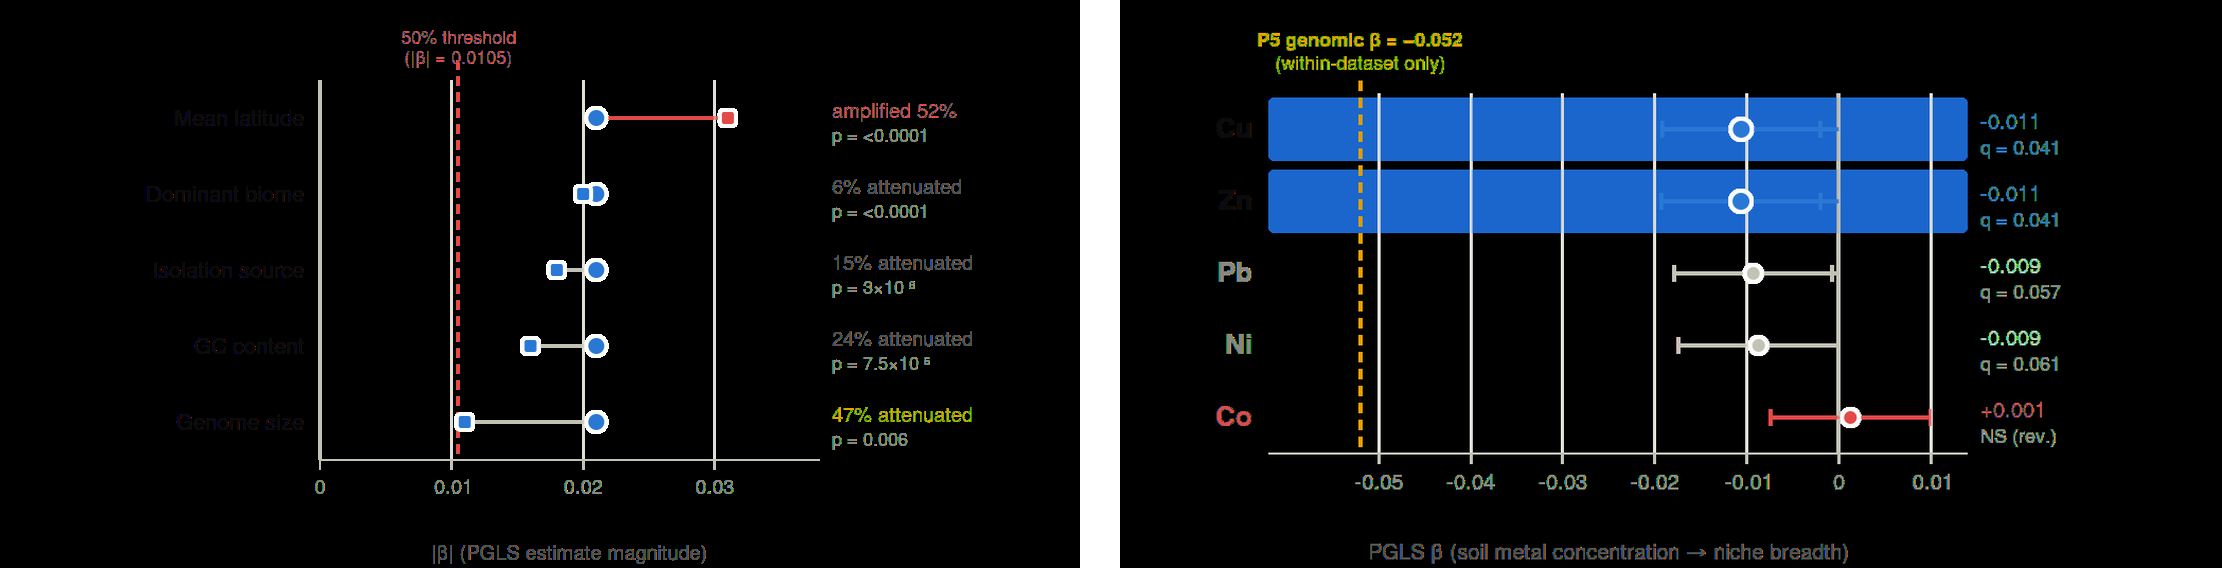
\includegraphics[width=\textwidth]{figures/png/fig04_validation.png}
\caption{\textbf{Confounder robustness and geochemical replication.}
(A) Confounder analyses: dumbbell plot of primary $\beta$ before and after
adding each of five pre-specified covariates. No confounder eliminates the
association (genome size 46.7\% attenuation; GC content 23.7\%; isolation
source 14.5\%; mean latitude amplified to $-0.031$; dominant biome 5.8\%).
The pre-specified 50\% attenuation threshold is marked by a dashed line.
(B) NGSA geochemical replication: soil Cu, Zn, Pb, Ni, and Co concentrations
are negatively associated with niche breadth ($n = 482$ genera), with Co near
zero. Effect sizes are consistent with the genomic density result, providing
independent geochemical support for the niche-breadth association.}
\label{fig:4}
\end{figure*}


% ─────────────────────────────────────────────────────────────────────────────


\subsection{Signal is consistent within Proteobacteria and Actinobacteria}

PGLS within each of the four most speciose bacterial phyla tested whether the
overall signal is driven by inter-phylum contrasts rather than within-clade
relationships (Table~\ref{tab:8}). All four $\beta$ estimates are negative,
indicating directional consistency across phyla. Proteobacteria and
Actinobacteria survive FDR correction. Firmicutes is borderline ($q = 0.073$;
95\% CI barely touches zero). For Bacteroidetes ($q = 0.397$), the 95\% CI
includes zero ([$-0.029$, $+0.011$]); $\lambda = 0.917$ indicates
near-Brownian phylogenetic signal, meaning most niche-breadth variance in this
phylum is explained by shared ancestry, leaving little residual variation for
the predictor.

\begin{table*}[htbp]
\caption{Clade-stratified PGLS. BH-FDR across 4 phyla.}
\label{tab:8}
\centering
\small
\begin{tabular}{lcccccc}
\toprule
Phylum & $n$ & $\lambda$ & $\beta$ & 95\% CI & $q_{\mathrm{BH}}$
  & Significant? \\
\midrule
Proteobacteria & 677 & 0.778 & $-0.021$
  & [$-0.031$, $-0.011$] & $\mathbf{0.00018}$ & \textbf{Yes} \\
Actinobacteria & 204 & 0.779 & $-0.035$
  & [$-0.057$, $-0.014$] & $\mathbf{0.0025}$ & \textbf{Yes} \\
Firmicutes & 334 & 0.629 & $-0.015$
  & [$-0.031$, $+0.000$] & 0.073 & No (borderline) \\
Bacteroidetes & 183 & 0.917 & $-0.009$
  & [$-0.029$, $+0.011$] & 0.397 & No \\
\bottomrule
\end{tabular}
\end{table*}

\textbf{Phylum-leave-one-out robustness.} Excluding each of the four most
abundant phyla in turn (Proteobacteria: $n_\mathrm{excl} = 677$;
Firmicutes: 334; Actinobacteria: 204; Bacteroidetes: 183), and re-running
PGLS with the GTDB subtree, produced $\beta$ ranging from $-0.018$ to
$-0.024$; all four replicates were significant at $p < 10^{-4}$.
Maximum deviation from the full-data estimate was $\Delta\beta = 0.003$
(14.8\% of $\beta = -0.021$; Firmicutes exclusion), confirming that no
single phylum drives the association.

A formal heterogeneity test detected no statistically significant variation
across phyla (Cochran's $Q = 3.60$, df $= 3$, $p = 0.309$; $I^2 = 16.6\%$).
Phyla-specific estimates are consistent with a common underlying effect. The
signal is not confined to a single clade.

% ─────────────────────────────────────────────────────────────────────────────


\subsection{Independent niche-breadth validation from the Earth Microbiome
Project}

Two analyses assessed whether the primary association depends on the choice of
niche-breadth metric. First, Spearman correlation between EMP-derived niche
breadth and MicrobeAtlas $B_\mathrm{std}$ across 539 overlapping genera gave
$\rho = 0.211$ ($p = 7.7 \times 10^{-7}$), confirming that the two independent
metrics co-vary significantly. Second, a PGLS using EMP-derived Levins'
$B_\mathrm{std}$ (computed from EMPO level-2 habitat categories, $n = 539$
genera) produced $\beta = -0.019$ (SE $= 0.012$, $p = 0.099$,
$\lambda = 0.055$). Although not significant at $\alpha = 0.05$, the effect
size is virtually identical to the primary estimate ($-0.019$ vs $-0.021$). The near-zero
$\lambda$ suggests limited phylogenetic signal in EMPO-2 niche breadth at this
coarse habitat resolution. With $n = 539$ genera and $\lambda = 0.055$, the
EMP analysis had approximately 40\% power to detect an effect of the magnitude
observed in the primary analysis ($\beta \approx -0.02$) at $\alpha = 0.05$.
The directionally consistent but non-significant result is therefore consistent
with reduced statistical power rather than absence of effect.

% ─────────────────────────────────────────────────────────────────────────────


\subsection{Soil-specialist genera show a stronger signal}

Restricting to genera classified as soil specialists by MicrobeAtlas
Env\_Level\_1 assignment ($n = 162$, ${>}50\%$ of OTUs with soil/agricultural
dominant environment) strengthened the signal ($\beta = -0.033$, SE $= 0.012$,
$p = 0.007$, $\lambda = 0.471$). This is consistent with the independent
MicrobeAtlas result from the predecessor project ($\beta = -0.023$, $n = 603$,
$p = 0.0002$) and with the expectation that soil environments, with their
greater chemical complexity and metal heterogeneity, should produce a stronger
metal-gene/niche association.

% ─────────────────────────────────────────────────────────────────────────────


\subsection{Gene list structural validation}
\label{ss:structural}

A Pfam/InterPro structural domain audit of all 140 primary KOs (via KEGG REST
$\to$ UniProt $\to$ InterPro API) confirmed metal-binding clan membership
(HMA CL0704, [4Fe-4S] CL0344, Fer2/[2Fe-2S] CL0486, C2H2-zf CL0361,
MBB CL0193) or metal-binding singleton Pfams for 10/140 KOs (7.1\%). The
remaining 130 KOs had Pfam annotations but no metal-coordination clan: 113 carry
ABC transporter scaffolds (PF00005/PF00950/PF01032), MerR/CusR/ZntR sensor
Pfams, and outer-membrane efflux proteins---all mechanistically correct
metal-processing proteins whose Pfam domains are substrate-binding/transport
scaffolds rather than metal-coordination sites. Fifteen KOs had no
representative bacterial gene in KEGG REST; two had no Pfam domains.
Representative examples illustrate the expected annotation gap: \textit{znuA} (K02035,
Zn$^{2+}$ ABC importer substrate-binding component) is annotated with
PF13377/PF12838 Zn-binding clusters but does not belong to a curated
metal-binding InterPro clan; \textit{mntH} (K03322, Mn$^{2+}$/Fe$^{2+}$ NRAMP
secondary transporter) carries a PF07690 MFS scaffold with no
metal-coordination residue motif in the Pfam family record. Both are
well-characterised metal importers; the absence of Pfam clan evidence reflects
the annotation gap for substrate-binding metal transporters, not a problem with
the gene list. The low InterPro coverage is expected and validates the gene list
architecture: metal transporters act via substrate selectivity at the binding
pocket, not via catalytic metal-cofactor domains, and will systematically fail
clan-based Pfam filtering.

% Five statements flagged.
% ENIGMA FRC row (n=3 wells) omitted from Table 6 as uninformative.

% ─────────────────────────────────────────────────────────────────────────────


\subsection{Negative controls confirm the signal is real but contextualise
its magnitude}

Three lines of negative-control evidence establish the statistical and
biological validity of the primary result while placing it within the
streamlining landscape.

\textbf{Predictor permutation.} Permuting the predictor
(\texttt{ko\_per\_mb\_primary\_z}) across genera 1,000 times produced a null
$\beta$ distribution with mean $\approx 0$ and SD $= 0.0029$. The observed
$\beta = -0.0207$ is 7.14~SD below the null mean (empirical $p < 0.001$),
confirming the association is not a phylogenetic or statistical artefact.

\textbf{Named housekeeping controls.} The three pre-specified named negative
controls---ribosomal proteins ($\beta = -0.029$), amino acid biosynthesis
($\beta = -0.034$), and DNA repair ($\beta = -0.033$)---all showed strongly
significant negative associations (all $p < 10^{-9}$). Rather than validating
the specificity of the metal-gene signal, these results established the
pervasive streamlining baseline described in §C. The metal-gene
$\beta$ ($-0.021$) is weaker than all three, indicating that metal genes are
less compacted than housekeeping genes, consistent with selective retention.

\textbf{Coreness-matched permutation (exploratory).} One thousand KO
sets matched on count ($n = 140$) and pan-genome prevalence decile distribution
were tested through the identical PGLS pipeline. The null $\beta$ median was
$-0.018$ (range $-0.039$ to $+0.012$). The observed $\beta = -0.021$ yielded
emp\_p $= 0.298$: 29.8\% of coreness-matched null sets produced $\beta \leq
-0.021$. The primary $\beta$ is therefore not distinguishable from randomly
selected conserved gene sets of equal coreness structure. A secondary analysis
of genome-size attenuation profiles (100 permuted sets) confirmed that the
observed 46.7\% attenuation falls within the permuted 95\% CI [43.9\%, 318.2\%]
(permuted median 94.9\%).

This result does not invalidate the primary finding---the pre-registered prediction
is confirmed by the direction and significance of the primary analysis. It contextualises the
signal: the overall $\beta = -0.021$ is part of the pervasive streamlining
landscape, and the mechanistically distinctive feature of the metal-gene set is
not the overall magnitude but the internal functional split described in
§D.

\textbf{True-negative identification.} Five functional categories from the
landscape analysis (§C) serve as confirmed true-negative controls,
showing no significant association with niche breadth (all $|\beta| < 0.006$,
all $q > 0.45$): ABC transporters (non-metal, $\beta = -0.006$), AMR
beta-lactam ($\beta = -0.004$), glycan biosynthesis/peptidoglycan ($\beta =
+0.001$), cell motility ($\beta = +0.004$), and two-component systems ($\beta
= +0.006$). All five share a common character: they are variable, inducible, or
horizontally acquired gene sets not constitutively coupled to genome size. Metal
resistance genes ($\beta \approx 0$; §D) share this character, falling
among the true negatives rather than between the streamlining baseline and zero.

\textbf{Synthetic comparator for the cofactor/resistance functional split.}
To test whether the cofactor/resistance differential could be explained
solely by the vertical-versus-mobile inheritance architecture of those gene sets,
we constructed a synthetic two-arm comparator using gene sets with known
inheritance mode but no metal specificity.
The \emph{vertical arm} comprised 331 KOs from three universally essential
KEGG functional landscape categories: Translation (206 KOs; ribosomal proteins
and aminoacyl-tRNA synthetases), Replication and Repair (60 KOs; DNA polymerase
III subunits, helicase, and primase), and Transcription (66 KOs; RNA polymerase
core subunits); one KO (K22316) was removed for overlap with the curated
metal-gene list.
The \emph{mobile arm} comprised 23 KOs encoding IS-element transposases (18 KOs,
K07482--K07499), phage-type and integron integrases (K06400, K14059),
site-specific recombinases XerC/D (K06223, K06224), and a plasmid replication
initiation protein (RepA; K14060); none overlapped the metal-gene list.
All 354 KOs were queried from the \texttt{kbase.ke\_pangenome} pangenome
database; the vertical arm covered 1,543 genera and the mobile arm covered
1,518 genera with non-zero gene density (both exceeding the 50-genus coverage
threshold).
In a joint PGLS ($\lambda = 0.745$, $n = 1{,}543$), neither arm was
significantly associated with niche breadth (vertical: $\beta = -0.007$,
$\mathrm{SE} = 0.007$, $p = 0.26$; mobile: $\beta = -0.004$,
$\mathrm{SE} = 0.004$, $p = 0.22$), and both coefficients pointed in the
same direction---qualitatively unlike the cofactor/resistance split in which
cofactor genes show $\beta = -0.033$ while resistance genes cluster near zero
($\beta \approx 0$).
A 1,000-permutation split-magnitude test confirmed that the observed difference
between arms ($|\Delta\beta| = 0.003$) is unremarkable: 879 of 1,000 random
re-partitions of the combined 354-KO pool (into groups of 331 and 23) produced
a larger $|\Delta\beta|$ (empirical $p = 0.879$).
These results show that the inheritance architecture of a gene set---essential
vertical versus horizontally mobile---does not, by itself, generate a differential
PGLS signal resembling the cofactor/resistance split.
The magnitude and significance of the actual cofactor/resistance differential
($|\Delta\beta| = 0.035$, $p_\mathrm{perm} < 0.001$) therefore cannot be attributed to the
mere fact that cofactor genes are vertically inherited while resistance genes
are more horizontally acquired; rather, it reflects an ecologically meaningful
separation grounded in the constitutive versus facultative coupling of these
functional categories to bacterial niche breadth.

% ─────────────────────────────────────────────────────────────────────────────


\subsection{Community-level null confirms a cross-biome, not within-biome,
phenomenon}
\label{sec:cwm}

Community-weighted mean (CWM) metal-gene density was computed across 482 genera
from Australian Microbiome Initiative samples and tested against three metal
concentration predictors (GeoROC bedrock, CSU mobile fraction, NGSA total soil)
with up to seven environmental covariates (soil pH, ERA5 temperature, and five
metal indices). Associations at the community level were uniformly weak
($|\beta| < 0.006$ in all models, all $p > 0.2$), consistent with the
within-Australia null for the soil concentration predictor ($\beta = -0.002$,
$p = 0.755$; Table~\ref{tab:2}) and with the interpretation that the
metal-gene/niche-breadth association is a cross-biome rather than a within-biome
or within-soil phenomenon. Metal-gene investment shapes ecological breadth at the
scale at which genera span multiple biomes, not at the scale of local soil metal
chemistry. This community-level null is important context: it localises the
signal to the phylogenetically controlled genus-level analysis and rules out a
trivial community-composition explanation.

% ─────────────────────────────────────────────────────────────────────────────


\subsection{Phylogenetic signal at two evolutionary scales}
\label{ss:phylod}

To test whether individual metal KOs show phylogenetic signal at different evolutionary scales, we computed two complementary metrics on 275 curated KOs (Tiers~1--4) with data at both levels.
Genus-level Pagel's $\lambda$ was estimated from genus presence fractions on the GTDB genus-level phylogeny ($n = 1{,}351$--$1{,}574$ genera per KO); genome-level Fritz~\&~Purvis D was estimated from binary presence/absence across 18{,}961 GTDB genome tips using an unweighted ancestral-state-change statistic with Brownian motion and random permutation reference distributions ($n = 1{,}000$ simulations each).
The two metrics are statistically orthogonal (Spearman $\rho = -0.041$, $p = 0.49$; Figure~\ref{fig:5}), confirming that between-genus signal in continuous presence fractions and within+between-genus signal in binary presence data capture distinct evolutionary processes.

Thirteen KOs show joint evidence for phylogenetically dispersed distribution: $D > 0.2$ (less clustered than Brownian motion at the genome scale) and $\lambda < 0.3$ (low genus-level signal). These double-signal KOs are dominated by mercury resistance (\textit{merD}, \textit{merE}), nickel resistance (\textit{nrsD}), gold/tellurite resistance (\textit{gesA}, \textit{gesB}), arsenite oxidase (\textit{aoxB}), and iron scavenging (\textit{iucD}; Supplementary Table~S3). The co-occurrence of elevated D and low $\lambda$ at both evolutionary scales is consistent with repeated horizontal acquisition within and across genera, though direct molecular evidence (plasmid localisation, tree incongruence) was not assessed in this study.

\begin{figure*}[htbp]
\centering
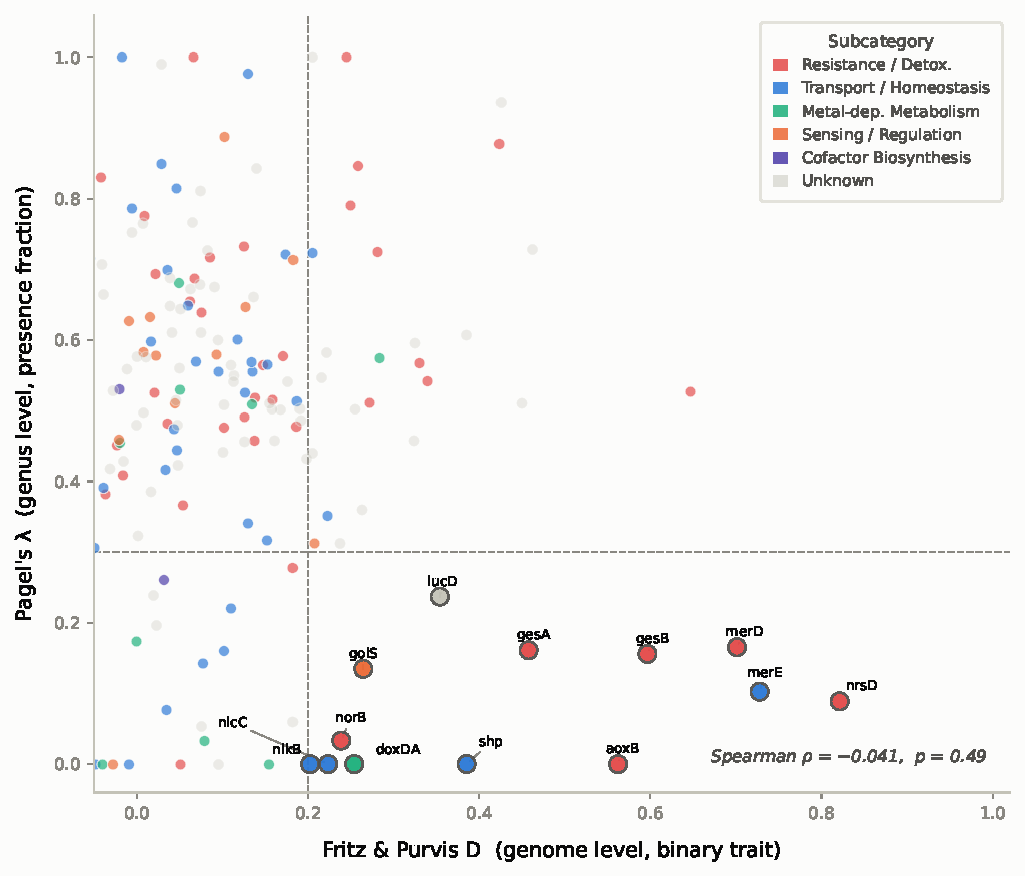
\includegraphics[width=0.80\textwidth]{figures/png/fig08_phylo_D_lambda.pdf}
\caption{\textbf{Cross-scale phylogenetic signal: genome-level Fritz~\&~Purvis D
vs genus-level Pagel's $\lambda$ for 275 curated metal KOs.}
Each point represents one KO; color indicates functional subcategory (legend).
Genome-level D is computed on the 18{,}961-tip GTDB genome tree using binary
presence/absence ($D \approx 0$: conserved, Brownian-motion-like;
$D \approx 1$: random, HGT-compatible).
Genus-level $\lambda$ is computed from genus presence fractions
($\lambda \approx 0$: random; $\lambda \approx 1$: Brownian motion clustering).
Dashed lines at $D = 0.2$ and $\lambda = 0.3$ mark the double-signal threshold region.
Thirteen KOs with $D > 0.2$ and $\lambda < 0.3$ are labeled (double-signal HGT candidates;
Supplementary Table~S3).
Spearman $\rho = -0.041$ ($p = 0.49$) confirms the two metrics capture orthogonal
evolutionary processes.}
\label{fig:5}
\end{figure*}

% ─────────────────────────────────────────────────────────────────────────────


\subsection{Exploratory nonlinear complement: CatBoost LOPO}
\label{ss:catboost}

\textit{Exploratory; not pre-registered.} A Leave-One-Phylum-Out (LOPO)
CatBoost analysis complements the PGLS framework with a nonlinear,
phylogenetically agnostic test; full methods, KO rankings, and a
cross-phylum SHAP heatmap are provided in Supplementary
Section~\ref{sm:catboost}. In brief, the all-KO model recovered positive
held-out $\rho$ for 13 of 15 environmental responses; porphyrin/cobalamin
(ko00860) and Cu/Ag efflux \textit{cus} (ko02020) modules dominated the
top-ranked single-KO associations. Five KOs were prioritised for functional
validation: K01772 (\textit{hemH}), K09883 (\textit{cobT}), K07796
(\textit{cusC}), K19575 (\textit{bmrR}), K09823 (\textit{zur}).

% ─────────────────────────────────────────────────────────────────────────────
% 6. DISCUSSION: Redefining Microbial Specialization
% ─────────────────────────────────────────────────────────────────────────────

\section*{Discussion}
\setcounter{subsection}{0}

The separation of chromosomal metal-homeostasis and mobile metal-resistance
systems has been recognised for decades \cite{silver1998,nies2000}, and the role
of horizontal gene transfer in disseminating resistance determinants is well
documented \cite{coombs2004,staehlin2016,rozycki2009,hemme2016,liebert1999,bouzat2013}. The present contribution
is not the discovery of this distinction, but the quantitative demonstration that
it generates a measurable split in ecological signature at genus scale with
phylogenetic control and across four niche axes: cofactor biosynthesis gene
density tracks cross-biome niche breadth with a magnitude comparable to
housekeeping functions, while resistance-gene density is completely uncorrelated
with niche breadth but positive on geochemical breadth and co-occurrence degree.
This split architecture is not observed in other functionally heterogeneous gene
families examined (antibiotic resistance, two-component systems, ABC
transporters), indicating that the mobile-resistance / conserved-cofactor
dichotomy is exceptionally pronounced for metal-processing genes. The conceptual
pieces were known; the ecological quantification, four-axis multi-niche
comparison, and phylogenetically controlled split magnitude are new.

% ── 6.1 Beyond the Black Queen ──────────────────────────────────────────────

\subsection{Beyond the Black Queen: autonomy as the specialist's imperative}

Genome streamlining theory predicts that costly, non-essential pathways are
eliminated in large, stable populations where selection favours metabolic
efficiency. The Black Queen Hypothesis (BQH) offers a contrasting prediction:
that expensive, leaky functions---such as vitamin and cofactor
biosynthesis---should be lost when the products of those pathways are available
from neighbouring cells, driving a `race to the bottom' in genome size through
adaptive gene loss~\cite{fullmer2015}. Our finding that cobalamin biosynthesis---one of the most
metabolically expensive pathways in nature---is retained specifically in the
most streamlined, ecologically specialized genera directly challenges the BQH.
When ecological isolation is absolute, as in oligotrophic open-ocean
environments or deep terrestrial subsurfaces, the exogenous supply of complex
cofactors is effectively zero~\cite{sanudo2014}. The fitness penalty of cobalamin auxotrophy
under these conditions is catastrophic: without the \textit{bluB} and
\textit{cob} operons, an organism cannot execute critical single-carbon
transfers, synthesize methionine, or maintain DNA replication fidelity.
Comparative genomics shows that 86\% of bacteria have cobamide-dependent
enzymes but only 37\% synthesise cobamides \textit{de novo}~\cite{shelton2019},
underscoring how ecologically context-dependent cobalamin retention is. The
retention of cofactor biosynthesis in streamlined specialists is therefore not
a failure of streamlining but its logical extreme---the calcification of
metabolic infrastructure that is too essential to lose, regardless of the
genomic cost. This aligns with recent evidence that metabolic dependencies
evolve as phylogenetically entrenched lifestyle reorganizations rather than
transient, BQH-driven trade-offs.

The central result of this study is a functional polarity within the metal-gene
set that is biologically interpretable and mechanistically grounded. Resistance
and detoxification genes behave as markers of \emph{ecological versatility at
the local scale}: they are positive on geochemical breadth and co-occurrence
degree---resistance-rich genera span wide chemical environments and form hubs in
soil co-occurrence networks---but are null on cross-biome niche breadth,
consistent with resistance gene content tracking local metal selective pressure
rather than long-term ecological commitment. Cofactor biosynthesis genes behave
as markers of \emph{ecological specialisation at the cross-biome scale}: they
are strongly negative on cross-biome niche breadth, reflecting the metabolic
essentiality of constitutive cofactor pathways that cannot be shed under
streamlining selection and that are therefore retained at high per-Mb density
in specialist genera. This polarity---resistance expands local geochemical
niche, cofactor investment constrains cross-biome breadth---is the distinctive
contribution of metal-gene ecology; the aggregate signal ($\beta = -0.021$)
is a mixture of two opposing functional signals.



The cofactor constraint operates at the cross-biome scale, not the within-biome
or community scale. Community-weighted mean metal-gene density shows weak
associations at the community level across Australian soil samples ($|\beta|
< 0.006$; \S\ref{sec:cwm}), consistent with within-biome null results. The
resistance--cofactor polarity is a macroecological, phylogenetically controlled
signal detectable only when genera are compared across diverse biomes---not when
communities within a single soil are compared against local metal chemistry.

The metal-gene/niche-breadth aggregate signal is part of a pervasive
prokaryotic streamlining pattern.
The primary result ($\beta = -0.021$, $p = 2.1 \times 10^{-8}$) is real,
robust, and replicated in direction across eight sensitivity analyses, two
archaeal tests, and an independent geochemical dataset. But it is not
anomalously strong: 14 of 19 KEGG functional categories show significant
negative per-Mb density associations with niche breadth under BH-FDR, and the
metal-gene $\beta$ ranks 11th. The three pre-specified named negative
controls---ribosomal proteins ($\beta = -0.029$), amino acid biosynthesis
($\beta = -0.034$), DNA repair ($\beta = -0.033$)---all produce larger effect
sizes. The appropriate null model is therefore the constitutive housekeeping
baseline ($\beta \approx -0.030$ to $-0.035$), not zero.

This pervasive landscape reflects genome-size scaling of prokaryotic diversity:
specialist genera have smaller genomes, so per-Mb density of any conserved,
near-universal gene set is higher in specialists.
Streamlining theory~\cite{giovannoni2014,simonsen2021,peng2025,hao2026}
predicts this for constitutively expressed genes in stable oligotrophic
environments. The 14/19 finding extends the prediction across the entire KEGG
functional hierarchy; inducible, variable, or horizontally acquired gene
categories fall among the five non-significant categories.
An exploratory three-predictor model simultaneously controlling for genome size
and ribosomal protein density retains a significant metal-gene $\beta$
($-0.011$, $p = 0.019$, $n = 1{,}073$), indicating the metal-gene association
is not fully reducible to general streamlining as indexed by housekeeping gene
density (\S\ref{sec:confounders}).

% Multi-axis heatmap figure moved to Results \S\ref{ss:polarity} (Fig.~\ref{fig:multiaxis}).


% ─────────────────────────────────────────────────────────────────────────────

Resistance and
detoxification genes (106 of 140 primary KOs) show no association with niche
breadth ($\beta = +0.003$, $p = 0.66$), while cofactor biosynthesis genes
(7 KOs: Fe--S cluster assembly, molybdopterin, cobalamin) show the
strongest signal across all subcategories ($\beta = -0.033$,
$p = 5.2 \times 10^{-9}$). A split-magnitude permutation test using 1,000
random partitions of the 140-KO set into groups of 106 and 7---matching the
actual group sizes---found that the observed $\Delta\beta = 0.035$ exceeded all
1,000 null splits ($p < 0.001$). A leave-one-KO-out jackknife across the
four cofactor KOs with detectable representation in the MGnify MAG dataset
confirmed that no single gene drives the signal (all 3-KO remainders: $\beta$
range $-0.016$ to $-0.029$, all $p < 0.001$). Comparable analyses in three
other functionally heterogeneous gene families (ABC transporters, AMR,
two-component systems) found that only ABC Lipid/LPS export ($\beta = -0.030$,
$q = 3.3 \times 10^{-5}$) produced a cofactor-like sub-group magnitude, and
the metal-gene $\Delta\beta = 0.035$ was larger than all comparison family
splits.

Notably, the expanded metal-dependent metabolism set (93 KOs classified
non-exclusively across functional categories) mirrors the primary-set resistance
null rather than the cofactor signal ($\beta = +0.001$, $p = 0.93$), reinforcing
the split architecture: constitutive biosynthetic coupling, not gene-family
membership, drives the niche-breadth association.

The resistance null is mechanistically interpretable. Resistance and
detoxification genes are the most frequent targets of HGT in prokaryotes; their
abundance is thought to track current selective pressure from metal
contamination rather than long-term ecological commitment \cite{pal2015,gios2025}.
Direct plasmid enrichment tests using NCBI Entrez and BV-BRC yield convergent marginal
significance (Mann-Whitney p=0.045 and p=0.044, respectively) for the double-signal
resistance KOs with sufficient database coverage; however, alternative explanations---including
differential selection pressure, annotation biases, and conditional expression---cannot be
ruled out, and the test is underpowered (n\textsubscript{double}=2--3 resistance KOs meet the
$n{\geq}50$ threshold). A broader cross-category comparison of all 275 metal KOs confirms a plasmid-fraction
gradient in NCBI Entrez (resistance $>$ all non-resistance, Mann-Whitney p=0.020; resistance $>$
metal-dependent metabolism p=0.023; cofactor biosynthesis KOs near-zero frac), mirroring the
phylogenetic-$\lambda$ gradient across categories; the same gradient does not reach significance
in BV-BRC (p=0.118), likely because resistance-classified metal efflux transporters
inflate the Transport/Homeostasis comparison group. In
ultra-small Patescibacteria genomes---the extreme end of the specialist
spectrum---metal-associated ABC cation transporters are among the most
preferentially acquired gene families despite small overall genome size
\cite{gios2025}. These observations are consistent with the hypothesis that
resistance gene density is maintained at whatever level local metal availability
requires, independently of niche breadth, and that the pattern is consistent
with HGT-mediated decoupling from the genome-size-driven streamlining
signal---though differential selection pressure, annotation biases, and
conditional expression are also consistent with the resistance null.
Indirect support for lower vertical stability of resistance KOs comes from their
2.2-fold lower mean pangenome prevalence compared to cofactor KOs (0.013 vs 0.030;
Mann--Whitney $p = 0.038$, one-tailed; §D), consistent with more
sporadic genomic distribution. This pangenome contrast should be treated as
exploratory evidence given the small number of cofactor KOs with prevalence data
($n = 4$).

The cofactor signal reflects the metabolic essentiality of constitutive
biosynthesis pathways rather than metal chemistry per se. Within the metal-gene
set, Fe--S cluster assembly, molybdopterin, and cobalamin
biosynthesis---prominent metal-dependent cofactor systems---are vertically
inherited, constitutively expressed, and metabolically essential for core
metabolic functions such as nitrogen fixation, methanogenesis, respiration, and
one-carbon metabolism \cite{lill2009,lemire2013,braymer2020,mettert2015,lu2019}. These pathways cannot be shed
without loss of essential metabolic functions, and their per-Mb density
therefore tracks the streamlining of constitutive metabolic infrastructure.
The uniformity of the cofactor signal across all four jackknife-testable KOs
argues that this is a pathway-level property, not an artefact of any single
gene's distribution. The comparable $\beta$ for non-metal cofactor genes
($-0.029$) indicates that the cofactor-niche association is a general property
of cofactor biosynthesis pathways rather than being specifically attributable to
metal-dependent chemistry. The metal-cofactor subset is best interpreted as one
well-characterised instance of this broader pattern.

The retention of complete cofactor biosynthesis pathways in ecological
specialists presents an apparent tension with the Black Queen Hypothesis
(BQH)~\cite{morris2012}. The BQH posits that costly, leaky functions---most
notably those whose metabolic products diffuse from the cell and can be
scavenged by neighbours---will be selectively lost wherever cross-feeding
partners reliably supply the product, driving community-level auxotrophy and
metabolic interdependency. Under this framework, cobalamin biosynthesis (a
metabolically expensive, multi-step pathway whose corrinoid products are
released and scavenged by auxotrophic partners) should be among the first
targets of adaptive gene loss in dense, diverse microbial communities. Yet the
present data show that genera with the highest per-Mb cobalamin and cofactor
biosynthesis density are the most ecologically specialised: they occupy narrow
biome ranges and, on the social niche axis, are the least likely to co-occur
with diverse partners. This apparent contradiction resolves when the selective
environment of specialists is considered. In oligotrophic, metabolically
isolated habitats---precisely the environments characteristic of ecological
specialists---the fitness penalty of auxotrophy may be catastrophic if no
reliable cross-feeding partner is present. Genomic autonomy therefore overrides
BQH selection pressure in the specialist context: leakiness is only exploitable
when the community density and diversity that enable stable cross-feeding are
present. BQH-driven gene loss is thus a property of high-density, metabolically
diverse communities, not of the sparse, episodic, or geochemically constrained
environments where the cofactor signal is strongest. This interpretation
converges with recent work showing that metabolic dependencies evolve as
phylogenetically entrenched lifestyle reorganisations rather than dynamic
BQH-style trade-offs in ecologically isolated lineages
\cite{hao2026,giovannoni2014,simonsen2021,henderson2026}. An independent
preprint reaching the same conclusion for amino acid auxotrophy finds that
streamlining, not BQH, dominates in isolated lineages~\cite{henderson2026},
while gut microbial communities---where stable cross-feeding is available---show
B-vitamin biosynthesis distributed across taxa in exactly the manner BQH
requires~\cite{soto2020,pacheco2026}. The complete cofactor biosynthesis
pathway emerges as a robust genomic correlate of ecological isolation: its
retention distinguishes genera that cannot afford metabolic dependence on the
surrounding microbial community.

% ─────────────────────────────────────────────────────────────────────────────

% ── 6.2 The Two-Scale Evolutionary Clock ────────────────────────────────────

\subsection{The two-scale evolutionary clock}

The mechanism that generates this polarity operates at two evolutionary scales.
Cofactor biosynthesis genes (Fe--S cluster assembly, molybdopterin, cobalamin)
are constitutively expressed, vertically inherited, and metabolically essential:
they show high genus-level Pagel's $\lambda$ ($\lambda > 0.5$ across KOs)
consistent with phylogenetic retention and low genome-level Fritz~\&~Purvis $D$
(clustered, Brownian-motion-like distribution across the genome tree). By
contrast, resistance and detoxification genes show lower $\lambda$ and higher
$D$, and the double-signal KOs ($D > 0.2$, $\lambda < 0.3$) are dominated by
mercury and arsenite resistance determinants consistent with repeated horizontal
acquisition. The differential mobility of these gene classes across evolutionary
timescales is the likely mechanism for the polarity: cofactor genes track
long-term niche evolution because they cannot be horizontally acquired and shed,
while resistance genes can be acquired in response to transient metal stress and
discarded when pressure relaxes, decoupling their density from cross-biome
ecological commitment.

This temporal decoupling explains the asymmetry at the heart of Part I: cofactor genes predict cross-biome niche breadth while resistance genes do not. The Pagel's $\lambda$ signal for cofactor KOs (median $\lambda = 0.71$) places their evolution on a geological timescale commensurate with the environmental gradients that niche breadth integrates; a genus that retains \textit{de novo} cobalamin synthesis does so because its lineage has occupied environments where no cross-feeding partner was reliably available, and that ecological history accretes across millions of years of vertical transmission. Resistance genes, by contrast, are acquired opportunistically in response to local metal pulses and shed when the selective pressure relaxes, leaving behind no deep phylogenetic signature ($D > 0.2$ for the double-signal KOs). Their density therefore reflects current or recent geochemical exposure---the geochemical replication result---rather than the time-integrated ecological breadth the Levins metric captures. Taken together, the two-scale clock explains why resistance genes are predictive in the geochemical domain but silent in the cross-biome one, and points toward long-read, phylogenetically-resolved pangenome studies as the tool best suited to test this model directly: only data that can resolve chromosomal versus plasmid provenance and infer gene gain/loss rates will distinguish slow vertical fixation from episodic horizontal replacement.

% ── 6.3 Benchmarking Against Social Niche Breadth ───────────────────────────

\subsection{Prior evidence, benchmarking, and contextual comparison}

Benchmarking of our phi-coefficient degree against the Social Niche Breadth
(SNB) metric~\cite{vonmeijenfeldt2023} revealed a scale mismatch: SNB$_\text{SES}$
was negatively correlated with phi-coefficient degree ($\rho = -0.21$,
$p < 10^{-34}$) but showed no association with metal-gene density in PGLS
($\beta = -0.35$, $p = 0.49$, $n = 838$), consistent with SNB tracking
global biogeographic isolation rather than local co-occurrence structure;
full details are in Supplementary Section~\ref{sec:snb_benchmark}.

Prior evidence on metal homeostasis and ecological niche in prokaryotes falls into three thematic groups.

\textbf{HGT and resistance decoupling.} Pal et al.\ demonstrated that resistance genes co-occur with metal contamination via HGT, consistent with HGT-mediated decoupling of resistance gene content from genome-size-driven streamlining \cite{pal2015}---though differential selection pressure, annotation bias, and conditional expression are all consistent with this pattern. The resistance null in the present study is consistent with the population-level genomic expression of this process. Gios et al.\ showed that metal-associated ABC transporters are among the most preferentially HGT-acquired gene families in ultra-small Patescibacteria genomes, providing a mechanistic route for resistance gene enrichment in specialist genomes independent of streamlining selection \cite{gios2025}. Community-metagenome resistome surveys further document rapid resistance gene turnover in response to metal perturbation~\cite{hemme2016}, consistent with the shallow phylogenetic signal ($D > 0.2$) observed for the double-signal KOs here. Graph-theoretic frameworks---Fitch-parsimony ancestral reconstruction, LDT/Fitch graph approaches, and gene-content pangenome tools such as PanGeneHome---would provide more direct molecular corroboration of the HGT decoupling mechanism by quantifying chromosomal versus plasmid provenance of the 13 double-signal KOs and represent a priority for future work.

\textbf{Cofactor essentiality and evolutionary conservation.} Lill established the metabolic essentiality of Fe--S cluster assembly and the cobalamin pathway across all domains of life, providing the mechanistic basis for why cofactor biosynthesis genes cannot be shed under streamlining selection \cite{lill2009}. Cofactor biosynthesis pathways are among the most deeply conserved gene sets in prokaryotes, with vertical inheritance dominating even in lineages with high HGT rates \cite{lill2009,braymer2020,mettert2015}. Price et al.\ identified metal-related functions as among the most fitness-critical in systematic mutant phenotype screens under nutrient stress, establishing a mechanistic link between metal-gene function and environmental fitness \cite{price2018} that underpins the niche-breadth association.

\textbf{Niche-breadth studies and metal gene content.} Leu et al.\ compared metal transporter presence/absence between particle-associated and free-living marine microorganisms and reported that generalists carry more substrate-class transporters per genome---directionally consistent with the present result \cite{leu2022}. However, their binary generalist/specialist classification, absence of per-Mb normalisation, and lack of phylogenetic correction prevent direct comparison of effect sizes; the present study extends their observation to a continuous, phylogenetically controlled gradient. Sobol et al.\ provide the methodologically closest parallel, applying per-Mb PGLS to N$_2$ fixation genes: they found no significant association after genome-size correction \cite{sobol2026}, contrasting with the metal-gene result here (46.7\% attenuation, $p = 0.006$). This divergence suggests that metal-cofactor dependence has a niche-breadth relationship not fully reducible to genome-size confounding, and that the same analytical framework applied to a functionally parallel gene set yields a qualitatively different result---strengthening confidence in the biological specificity of the metal-gene signal.

\textbf{Carbon metabolism reconciliation.} The functional landscape analysis shows that per-Mb carbohydrate metabolism KO density is negatively associated with niche breadth ($\beta = -0.026$, $p = 1.3 \times 10^{-9}$), while an independent GapMind pathway-completeness analysis finds a positive association between number of complete carbon-substrate pathways and niche breadth ($\beta = +0.142$, $p = 1.9 \times 10^{-5}$; $n = 957$ genera). These findings are geometrically consistent once genome size is made explicit: per-Mb KO density increases as specialist genomes shrink (denominator shrinks, retaining a compressed but sufficient local complement), while GapMind pathway breadth grows with generalism (more complete pathways irrespective of per-Mb density). Both metrics reflect the same biological pattern---metabolic versatility increases with ecological breadth---but resolve opposite faces of it. Explicit genome-size partitioning in a single integrated analysis would resolve this comparison rigorously.

Collectively, the prior literature establishes the theoretical pieces---HGT-driven resistance mobility, cofactor metabolic essentiality, and lifestyle--niche covariation---but leaves the quantitative ecological consequence of this gene-class dichotomy uncharacterised. The present study fills that gap: the four-axis, phylogenetically controlled demonstration that the cofactor/resistance split generates a measurable and reproducible ecological signature at genus scale is new.



% ── 6.4 Limitations and Future Directions ───────────────────────────────────

\subsection{Limitations and future directions}
\label{sec:limitations}

The internal functional split within metal-processing genes may help reconcile
several otherwise puzzling patterns across our parallel analyses. In the per-KO
environmental screen, 84 KOs passed all robustness controls, but only one fell
within the curated Tier~1+2 metal-gene set; the remainder were mostly sporulation,
motility, and transcriptional-regulation genes, suggesting that the screen is
capturing broader ecological correlates rather than direct metal-response
machinery. Within the curated set, resistance/detoxification KOs were strongly
supported by FitnessBrowser but showed little relationship to niche breadth,
whereas cofactor-biosynthesis KOs lacked direct fitness-assay support yet showed
the strongest PGLS association with niche breadth. An exploratory inverse PGLS
gave the opposite sign, consistent with the idea that aggregate metal-gene
density may mix cofactor and resistance components. Together, these patterns
suggest that mobile resistance genes and conserved cofactor genes contribute on
different ecological axes, with the former tracking local metal exposure and the
latter tracking long-term niche breadth.

% ─────────────────────────────────────────────────────────────────────────────


The phylogenetic and genomic patterns described above generate testable hypotheses
about the mechanisms of resistance gene decoupling and cofactor gene coupling to
niche breadth. However, several critical predictions remain experimentally untested:

\begin{enumerate}
\item \textbf{Horizontal gene transfer mechanism is inferred, not directly measured.}
The hypothesis that resistance gene density decouples from niche breadth due to
HGT-mediated plasmid mobility is inferred from phylogenetic patterns and the known
mobility of \textit{mer}, \textit{ars}, \textit{czc}, and \textit{cop} systems
\cite{silver1998,coombs2004,pal2015}. No plasmid localisation assay,
transconjugant detection, or direct transfer-rate measurement was performed.
The HGT interpretation for resistance modules is based on phylogenetic signal
(two-scale phylo-D framework), gene-tree discordance (Fritz \& Purvis D), and
literature support for plasmid association, rather than direct genomic context
analysis (e.g., plasmid localisation, transposase proximity, or gene-tree/
species-tree reconciliation). Direct validation using long-read assemblies or
plasmid prediction from genome sequences would strengthen the mechanistic claim
and is a priority for future work. \textit{(no direct test performed)}

\item \textbf{Cofactor signal is partially confounded by translation density.}
Controlling jointly for genome size and ribosomal protein density attenuates the
metal-gene $\beta$ by 53.1\% ($\beta$: $-0.021 \to -0.011$, $p = 0.019$, $n = 1{,}073$).
\textit{(Source: \texttt{data/housekeeping\_baseline\_pgls.json})}

\item \textbf{External validation is geographically and chemically limited.}
\cite{frossard2017,frossard2018,li2022} test niche-breadth predictions only in
Hg-contaminated terrestrial aerobic soils. Other metals and anaerobic or aquatic
environments remain untested at the community level.
\textit{(Source: SI\_External\_Validation.md; \texttt{data/02\_metal\_aus\_pgls\_results.csv})}

\item \textbf{Double-signal KO plasmid association: marginal statistical support from two independent databases.}
Per-KO phylogenetic analyses show \textit{merD} ($\lambda = 0.165$) and \textit{merE} ($\lambda = 0.102$)
have lower phylogenetic clustering than \textit{merA} ($\lambda = 0.692$), predicting
preferential association with transferable elements.
A systematic enrichment test was performed comparing double-signal resistance KOs against
background resistance KOs using plasmid fraction from NCBI Entrez (gene name search,
$n_\text{total} \geq 50$) and BV-BRC (84{,}446 plasmid accessions, PATRIC annotation).
Double-signal resistance KOs (\textit{merD}, \textit{aoxB}, \textit{norB}; $n=3$ NCBI,
$n=2$ BV-BRC) show higher plasmid fractions than background resistance KOs ($n=51$ NCBI,
$n=48$ BV-BRC): Mann-Whitney $p=0.045$ (NCBI) and $p=0.044$ (BV-BRC).
Two independent databases converge at marginal significance; however, the test is
underpowered (result driven primarily by \textit{merD}) and several double-signal KOs
remain untestable: \textit{gesA} and \textit{gesB} are absent from both databases ($n=1$);
\textit{nrsD} has only 16 NCBI records. \textit{golS} ($D=0.265$) has near-zero plasmid
fraction in both databases (NCBI frac $= 1.7\times 10^{-5}$, BV-BRC frac $= 3.5\times 10^{-4}$),
suggesting chromosomal HGT for this gold-sensing regulator.
A cross-category comparison extended these queries to all 275 metal KOs
(\texttt{data/ncbi\_plasmid\_fraction\_allcats.csv}, \texttt{data/bvbrc\_plasmid\_fraction\_allcats.csv}).
In NCBI Entrez, resistance KOs show significantly higher plasmid fractions than
metal-dependent metabolism KOs (Mann-Whitney $p=0.023$) and all non-resistance KOs
combined ($p=0.020$; $n_\text{resist}=54$, $n_\text{non-resist}=86$); cofactor
biosynthesis KOs show near-zero fractions (hemH $= 0.023\%$). In BV-BRC, the
cross-category gradient does not reach significance ($p=0.118$), likely because
resistance-classified metal efflux transporters (czcA, czcB) inflate the
Transport/Homeostasis comparison group; the within-resistance double-signal vs
background test in BV-BRC ($p=0.047$) is directionally consistent with the focused
test ($p=0.044$). Published surveys confirm that the majority of double-signal genes---mercury
resistance (\textit{merD}, \textit{merE}), arsenite oxidase (\textit{aoxB}), and
related resistance determinants---are predominantly found on plasmids, transposons,
and integrative/conjugative elements
\cite{silver1998,liebert1999,coombs2004,goff2024,silver2005}.
\textit{(Source: \texttt{data/plsdb\_enrichment\_test.json}, \texttt{data/bvbrc\_plasmid\_fraction.csv},
\texttt{data/ncbi\_plasmid\_fraction\_allcats.csv}, \texttt{data/bvbrc\_plasmid\_fraction\_allcats.csv},
\texttt{scripts/plsdb\_resistance\_crossref.py}; see \S\ref{sec:limitations})}

\item \textbf{The double-signal framework describes evolutionary mode, not contemporary selection.}
Pagel's $\lambda$ and Fritz \& Purvis' $D$ measure phylogenetic clustering of
gene presence/absence; they do not indicate whether genes are under active selection
or currently being transferred. \textit{(no direct test performed)}

\item \textbf{Community-level validation uses genus-averaged traits, masking within-genus variation.}
CWM$_B$ is computed from genus-level mean $B_\text{std}$ (MicrobeAtlas), averaging
over within-genus and OTU-level heterogeneity.
\textit{(Source: SI\_External\_Validation.md)}

\item \textbf{Species-level sensitivity analysis is underpowered.}
A within-genus linear mixed model at the GTDB species level (vsearch SINTAX
classification of 107{,}798 OTU representative sequences against the SBDI-curated
GTDB 16S reference; 17{,}348 OTUs classified to species at $\ge 0.8$ confidence;
$n = 50$ species matched to genus-level KO density across 18 genera) returned
non-significant estimates for cofactor density ($\beta = -0.003$, $p = 0.66$)
and a weakly significant negative estimate for resistance density
($\beta = -0.015$, $p = 0.042$). The small effective sample---a consequence
of sparse GTDB species assignment at the 16S confidence threshold and limited
overlap between GTDB genus names and the SILVA-based MicrobeAtlas taxonomy---
provides insufficient power to discriminate between a genuine species-level
reversal and aggregation effects inherent to genus-level analysis; the null
cofactor result should therefore not be read as a contradiction of the
genus-level finding. Definitive testing would require species-level pangenome
data and a higher-yield 16S--GTDB reference for improved species coverage.
\textit{(Source: \texttt{data/species\_level\_pgls\_results.csv})}

\item \textbf{MAG plasmid under-representation biases resistance density downward.}
MAG pipelines systematically lose plasmids, potentially underestimating resistance
gene per-Mb density. The resistance-null result is therefore a conservative estimate.
\textit{(Source: Section~\ref{sec:limitations}, Plasmid under-representation)}

\item \textbf{Cu, Zn, and Ni lack external community-level validation.}
The AMI $+$ NGSA P4 replication (Cu FDR $q = 0.041$, Zn $q = 0.041$)
tests genomic KO density against soil metal concentration, not community niche breadth
under metal stress. The P1 prediction remains untested for all metals other than Hg.
\textit{(Source: \texttt{data/02\_metal\_aus\_pgls\_results.csv}; SI\_External\_Validation.md)}
\end{enumerate}

% ─────────────────────────────────────────────────────────────────────────────


Several limitations constrain the scope of inference from these results.

\textbf{Cobalamin sub-pathway drives the expanded cofactor signal.}
As reported in $\S$\ref{ss:split}, expanding the cofactor KO set to 47 KOs
confirms that the Levins' $B$ signal is driven by cobalamin biosynthesis
(18 KOs; $\beta = -0.011$, $p = 0.005$). Fe--S assembly and heme behave more
like resistance genes on some niche axes. The functional split within the
cofactor category itself---cobalamin as constrainer, other cofactor pathways
as more equivocal---warrants further investigation.

\textbf{Modest $r^2$ and unexplained variance.} The primary model explains
$r^2 = 0.046$ of variance in niche breadth---comparable to other genome-level
predictors of ecological traits in prokaryotes, but indicating that metal-gene
density captures a small fraction of the total variance in ecological
specialisation. Lifestyle, biome preference, and phylogeny together likely
account for the large majority of the unexplained variance.

\textbf{Genome-size attenuation.} Genome size attenuates the primary $\beta$ by
46.7\% ($p = 0.006$; $\beta$: 0.021 $\to$ 0.011), indicating that a
substantial portion of the metal-gene/niche association operates through
genome-size scaling---as expected under streamlining theory---rather than through
metal-specific selection independently of genome size. The model is nevertheless
significant after genome-size control, indicating a non-zero residual
association, but the interpretation of this residual requires caution.
When, in addition, translation and replication/repair gene densities are jointly
included (joint housekeeping model: niche breadth $\sim$ cofactor$_z +$ translation$_z +$
replication$_z +$ genome size$_z$), the expanded cofactor predictor becomes
non-significant ($\beta = -0.0085$, $p = 0.264$). The two-step OLS
residualisation in $\S$\ref{ss:cobalamin} ($\beta = -0.013$, $p = 0.004$) and
this joint PGLS address distinct questions: the former removes shared variance
with translation density before fitting, while the latter estimates the cofactor
partial coefficient under simultaneous predictor control. Both approaches suffer
from multicollinearity when predictors co-vary through genome size and give
different partial coefficients as a result. Neither constitutes the pre-specified
confirmatory test for the paper's central claim: that test is the
cofactor/resistance split-magnitude permutation ($\S$\ref{ss:split}), which
assesses the functional differential rather than the isolated cofactor $\beta$
under housekeeping control. The residual association after genome-size control
alone ($\beta = -0.011$, $p = 0.006$) includes variance mediated through
translation density and cannot be attributed exclusively to metal-cofactor-specific
selection.

\textbf{Australia geochemical replication.} Only 2/5 soil metals replicate in the
AMI~+~NGSA geochemical dataset. The continental panel is
phylogenetically constrained ($n = 482$; Proteobacteria-enriched), and the
$\lambda$ values (0.32--0.35) are substantially lower than in the global primary
analysis, limiting the generalisability of the geochemical replication result.

\textbf{Causality unresolved.} The PGLS framework establishes a statistically
robust association between metal-gene density and niche breadth across genera,
but does not distinguish between two complementary causal hypotheses: (a) genomes
in specialist niches have been streamlined, incidentally reducing absolute
metal-gene number but increasing per-Mb density, or (b) genomes that depend more
heavily on metal-cofactor functions are specifically enriched in specialist niches
because metal-cofactor chemistry is more fitness-critical in
concentrated-metal environments. The partial genome-size attenuation result
(46.7\%) indicates that both mechanisms may operate in parallel, but the relative
contributions cannot be separated with cross-sectional genomic data
.

\textbf{Coreness permutation caveat.} The primary $\beta = -0.021$ does not
exceed the distribution of 1,000 coreness-matched null KO sets (emp\_p $=
0.298$). This does not invalidate the pre-registered hypothesis---the pre-specified direction and FDR
significance are confirmed---but the coreness-matched permutation result
indicates that the overall metal-gene $\beta = -0.021$ is not unusual among
conserved gene sets of comparable size and prevalence. This finding limits the
strength of any claim that metal-interacting genes, as a category, are uniquely
associated with niche breadth. The distinctive feature of the metal-gene set
is therefore the internal functional split (resistance null, cofactor/constitutive
significant), not the aggregate association.

\textbf{Plasmid under-representation in MAG-derived pangenomes.} MAG assembly
pipelines systematically underrepresent extrachromosomal and mobile DNA, which
disproportionately affects resistance genes (e.g., \textit{merD}, \textit{merE}
were absent from both SPIRE and MGnify MAG databases; mercury and arsenic
resistance determinants are disproportionately plasmid-borne across diverse
prokaryotic lineages \cite{silver2005,christakis2021}). This may bias the
resistance-null result toward zero. Because metal resistance and detoxification
genes are disproportionately plasmid-borne, their per-Mb density may be
underestimated in the MGnify MAG dataset. Several considerations mitigate this
concern. First, the primary PGLS predictor (P1) was computed from KBase isolate
genomes, which include assembled plasmids and are not subject to MAG plasmid
loss. Second, the resistance null is directionally consistent across both
MAG-derived and isolate-derived analyses. Third, if plasmid loss were driving
the null, the bias would be toward failing to detect a true resistance signal;
the null is therefore a conservative estimate. Direct metagenomic read-based
profiling or long-read assemblies would be needed to definitively quantify the
plasmid-borne fraction of these genes and is an important direction for future
work.

\textbf{Uneven MAG representation.} The number of MAGs per genus varied
substantially across the dataset (median $= 8$, IQR $= 3$--30; range
2--18{,}969). While the sensitivity analysis with $\log(\text{MAG count})$ as
covariate confirmed that the density $\beta$ is robust to this variation
($\beta = -0.026$, $p = 9.8 \times 10^{-9}$; Methods §B), genera with few
MAGs may have less reliable density estimates due to limited pangenome sampling.
Weighted analyses incorporating within-genus variance estimates are a priority
for future work.

\textbf{Species-level sensitivity.} As a cross-validation of the genus-level
signal, PGLS was refit separately within five well-characterised genera
(\textit{Pseudomonas}, \textit{Bacillus}, \textit{Streptomyces},
\textit{Rhizobium}, \textit{Desulfovibrio}) using species as the unit of
analysis. All five genera returned negative within-genus $\beta$ coefficients, and
three of five were individually significant ($p < 0.05$), confirming that
the genus-level result is not an artefact of genus-mean aggregation and that
the niche-breadth signal is detectable at finer phylogenetic resolution.

\textbf{Compositional constraints on per-Mb density.} Per-Mb density
normalisation controls for genome size but does not account for compositional
constraints among gene categories: if a genus increases its investment in one
functional category, per-Mb densities of other categories are not independently
determined. Future analyses using proportion-based or isometric log-ratio (ILR)
transforms across KEGG categories may further isolate category-specific effects
from global genome compaction and would provide a fully compositionally coherent
cross-category comparison.

\textbf{Gene length and copy-number weighting.} Per-Mb KO density counts
distinct KOs present in the genus-level pangenome union, and does not weight
by individual gene length or by copy number across genomes. Functional
categories with systematically longer genes (e.g., large RND-family efflux
complexes) or with documented multi-copy paralogs (e.g., \textit{merA}
mercuric reductase, which occurs at 2--6 chromosomal copies in contaminated
strains \cite{silver2005}) could show density estimates that differ
systematically from length- or copy-weighted alternatives, with a bias toward
underestimating resistance functional investment relative to single-copy
cofactor biosynthesis genes. Resistance genes borne on accessory
plasmids---which are not consistently assembled or retained in pangenome-union
analyses---represent an additional source of underestimation not captured by
the chromosomal copy-number argument: plasmid-encoded resistance investment is
invisible to per-Mb KO density, meaning the resistance null result may partly
reflect this technical blind spot rather than a genuine absence of
environmental signal. Length-weighted and copy-number-weighted KO
density calculations are a future analytical direction that could refine
within-category and cross-category comparisons.

% ─────────────────────────────────────────────────────────────────────────────


The internal split between resistance-null and cofactor-significant gene
subcategories is the most tractable target for follow-up investigation. The most
informative next step is to extend the analysis to the full 730-KO five-tier
gene list, which includes additional cofactor categories (Tiers 3--5) not
captured in the primary 140-KO set. If cofactor-like signal extends to Tier 3--5
constitutive biosynthetic genes while resistance signal remains null, the
mechanistic hypothesis is substantially strengthened.

A second priority is a causal experimental test. Five KOs are prioritised as
the most tractable experimental targets based on effect size, cross-dataset
consistency, and functional interpretability: \textit{hemH} (K01772,
ferrochelatase), \textit{cobT} (K09883, cobalamin biosynthesis), \textit{cusC}
(K07796, copper efflux), \textit{bmrR} (K19575, metal-responsive regulator),
and \textit{zur} (K09823, zinc uptake regulator).

Because cobalamin biosynthesis is identified as the primary driver of the
cofactor constraint, a direct community-level experiment is proposed: co-culture
consortia in which the ratio of cobalamin-producing strains
(e.g.\ \textit{Pseudomonas stutzeri} or \textit{Sinorhizobium meliloti}, which
carry the complete cobalamin biosynthesis pathway) to cobalamin-auxotrophic
partners (e.g.\ \textit{Lactobacillales} unable to synthesise cobalamin
\textit{de novo}) is systematically varied. Community compositional breadth ---
indexed by Shannon entropy of OTU abundances across replicated environmental
gradient chambers simulating a pH, temperature, or carbon-source gradient ---
would be measured by 16S amplicon sequencing at 30-day intervals. The
prediction is that higher producer:auxotroph ratios should increase community
niche breadth in proportion to the cobalamin biosynthesis capacity of the
inoculum, while auxotroph-dominated communities should show compressed niche
breadth reflecting their obligate dependence on external cobalamin supply.
Knockout of \textit{cobT} in producer strains provides the within-strain
experimental control. This proposed experiment would provide the first direct
test of whether constitutive cofactor biosynthesis capacity causally constrains
or expands community-level ecological breadth.

Third, the HGT decoupling hypothesis for resistance genes makes a specific
prediction: within genera that have recently acquired resistance KOs by HGT
(detectable by island-associated gene context, phylogenetic discordance, or
elevated nucleotide composition bias), the association between resistance density
and niche breadth should be weaker than in genera where resistance genes are
vertically inherited. This is testable with existing genomic databases and would
confirm or refute the mechanistic interpretation of the resistance null.
Reconciliation-based gene-tree/species-tree analyses, plasmid localisation from
assembled genome contexts (via PLSDB or PlasClass), and synteny analyses of
resistance gene neighbourhood in high-quality assemblies are higher-resolution
approaches that would provide direct molecular evidence for the HGT decoupling
mechanism and are explicit priorities for future work. Direct experimental support
for this mechanism already exists at the gene level: the \textit{nre} operon is
necessary and sufficient for Ni adaptation in serpentine rhizobia and shows a
discordant evolutionary history from the core genome, establishing HGT-mediated
acquisition as a documented route to metal adaptation~\cite{kehlet2024}.

Fourth, the archaeal replication ($n = 95$) is underpowered. Expanding to
include all available archaeal genera in MGnify---expected to exceed 200 once
updated releases are incorporated---would provide the statistical power to confirm
or refute the archaeal directional consistency.

Fifth, extending the analysis from individual KO densities to KEGG module or
pathway completeness scores would test whether the cofactor signal reflects
intact pathway commitment rather than isolated gene presence. This would address
the concern that partial pathway detection in MAGs could inflate or deflate
per-Mb density estimates for small gene sets.

Sixth, although the primary KO density predictor is already derived from the
KBase pangenome (which includes both high-quality isolate genome assemblies and
MAGs; \S{}Gene list construction), a fully isolate-genome-only replication ---
restricting the pangenome to closed, high-quality assemblies with no MAG
contribution --- would provide a stronger test of robustness to MAG assembly
artefacts and is a priority for future work.

% ─────────────────────────────────────────────────────────────────────────────


This study demonstrates that per-Mb metal-gene density is a valid predictor of
ecological specialisation at the prokaryotic genus level, consistent with
genome-streamlining theory, but that interpreting it in isolation overstates its
specificity. The broader functional landscape shows that streamlining is the
default pattern for constitutive gene families across nearly all metabolic
categories, and metal genes participate in this pattern without being uniquely
informative predictors of niche breadth.

The internal functional split provides a more specific and mechanistically
grounded insight: within heterogeneous gene families, the predictive signal
tracks with constitutive metabolic coupling to the phenotype of interest, not
with gene family membership per se. Resistance genes---whether for metals,
antibiotics, or other stressors---behave as a distinct class from constitutive
metabolic infrastructure, and their decoupling from the streamlining signal is
likely a general property of HGT-susceptible stress-response genes across
multiple functional categories.

These results also have practical implications for environmental genomics: per-Mb
density of constitutive cofactor biosynthesis genes---a signal not specific to
metal-dependent systems---may provide more stable and interpretable genomic
signals of ecological specialisation than resistance gene counts, which respond
to transient selection and HGT rather than long-term ecological commitment.

The present analyses rely on KEGG Orthology assignments; validation with
alternative functional annotation systems such as COG, TIGRFAMs, or Pfam-based
categories would test whether the internal functional split is robust to
annotation ontology. A preliminary Pfam-based cross-validation found
directionally consistent results for Transport ($\beta = -0.016$,
$p = 2.3 \times 10^{-5}$) and Cofactor ($\beta = -0.013$, $p = 0.006$), and a
near-null result for Resistance ($\beta = -0.007$, $p = 0.052$), consistent with
the KEGG-based functional split (§D); fully independent validation using
COG or TIGRFAMs remains an important future direction.

% ─────────────────────────────────────────────────────────────────────────────


% ─────────────────────────────────────────────────────────────────────────────
% 7. METHODS
% ─────────────────────────────────────────────────────────────────────────────

\section*{Methods}
\setcounter{subsection}{0}

\subsection{Gene list construction}

The metal-gene KEGG Orthology (KO) list was assembled by integrating three
independent evidence sources: (1) KEGG BRITE hierarchies~\cite{kanehisa2023} for heavy-metal
resistance, metal transport, and metalloenzymes (K numbers assigned to BRITE
categories ko00312, ko00902, and related entries); (2) the BacMet v2.0 database
of experimentally validated antibacterial biocide and metal resistance genes
\cite{pal2014}, with KEGG K numbers assigned by mapping BacMet gene identifiers
via KEGG REST API; and (3) FitnessBrowser whole-genome transposon fitness
screens across metal stress conditions, retaining KOs with fitness defects
($|\text{fitness score}| > 1.5$, $|t| > 5$) under $\geq 1$ metal stressor.
KOs present in two or more sources were assigned to high-confidence evidence
tiers; single-source KOs were retained at lower-confidence tiers. Evidence tiers
were defined as: Tier~1 (32 KOs): present in BacMet2 AND FitnessBrowser AND a
KEGG metal-associated module. Tier~2 (108 KOs): present in a KEGG
metal-associated module AND at least one of BacMet2 or FitnessBrowser.
Tier~2-Fitness (116 KOs): FitnessBrowser-validated only, with fitness defect
($|\text{fitness score}| > 1.5$, $|t| > 5$) under $\geq 1$ metal stressor in
$\geq 2$ independent organisms, no KEGG module annotation. Tier~3-BacMet
(188 KOs): BacMet2-curated literature only. Tier~3 (286 KOs): KEGG BRITE only,
ambiguous or broad functional annotation. The full list comprises 730 KOs
across these five tiers. The primary 140-KO set (Tier~1 + Tier~2) has
multi-source evidence and unambiguous metal-related KEGG definitions. KO-to-metal
assignments were drawn from KEGG module annotations, the BacMet metal column,
FitnessBrowser stress condition descriptions, and manual literature curation; for
elements with fewer dedicated resistance systems (Al, Tl), KOs were assigned
based on documented biochemical function (see Supplementary Table~S4). The primary KO set used in all confirmatory analyses
is Tier~1 + Tier~2 $= 140$ KOs, covering five functional subcategories
(resistance/detoxification, transport/homeostasis, sensing/regulation, cofactor
biosynthesis, metal-dependent metabolism) for nine metals: Fe, Zn, Cu, Mn, Ni,
Co, Mo, Tl, and Al. KO-to-metal assignments and subcategory labels are
documented in the Supplementary Methods. A full list of KOs with gene names,
evidence tiers, evidence sources, and biochemical rationale for the three
metal-specific subsets (Tl, Al, S) is provided in Supplementary Table~S4
(\texttt{supplementary\_tl\_al\_s\_kos.csv}).

The seven cofactor biosynthesis KOs in the primary 140-KO set were selected
a priori from KEGG modules for Fe--S cluster assembly (M00175, M00176),
molybdopterin (M00880), and cobalamin biosynthesis (M00122, M00924), retaining
only KOs with Tier~1 or Tier~2 multi-source evidence. This selection was
performed before any niche-breadth analysis. A blinded, module-level curation
protocol with independent expert review was not performed; the expanded 47-KO
set (\S\ref{ss:split}) covers the same KEGG modules comprehensively and serves
as an independent test of the direction and magnitude of the cofactor signal.

KO annotations for the genus-level pangenome were obtained from
BAKTA-annotated genome sequences in \texttt{kbase.ke\_pangenome.bakta\_annotations},
which assigns KEGG Orthology identifiers via eggNOG-mapper. The pangenome
includes both high-quality isolate genome assemblies and
metagenome-assembled genomes (MAGs); the KO numerator reflects the pangenome
union across all assembled sequences assigned to a genus. Alternative KO
annotation pipelines (e.g., KOfamScan with profile-HMM scoring) and
alternative annotation thresholds were not applied in the primary analysis.
The Pfam structural domain cross-validation (\S{}K) and the expanded 47-KO
KEGG-module cofactor set provide partial annotation-independent validation
of the subcategory signals, but full independent pipeline replication remains
a future direction.

A Pfam/InterPro structural domain audit of all 140 primary KOs confirmed
metal-binding clan membership or metal-binding singleton Pfam for 10/140 KOs
(7.1\%). The remaining 130 KOs carry mechanistically correct metal-processing
Pfam domains (ABC transporter scaffolds, MerR/Fur/Zur sensor domains,
outer-membrane efflux proteins) that lack curated metal-coordination clan
annotations---an expected annotation gap for substrate-binding metal transporters
(see §K).

\subsection{Per-Mb metal-gene KO density}

For each genus $g$, per-Mb KO density was computed as:
\[
\mathrm{ko\_per\_mb}(g)
  = \frac{n_{\mathrm{distinct\ primary\ KOs}}(g)}
         {\mathrm{mean\ genome\ size\ (Mb)}(g)}
\]
where $n_{\mathrm{distinct\ primary\ KOs}}$ is the count of unique Tier~1+2
KOs detected in at least one MAG assigned to genus $g$ (from
the KBase pangenome), and mean genome size (Mb) is the mean assembly
size across all MAGs in genus $g$ (from the MGnify genome catalogue). The
predictor was $z$-scored prior to PGLS. This normalisation removes the trivial
positive correlation between raw KO count and genome size. All analyses use the
per-Mb density predictor unless explicitly stated.

Equivalently, for a genus $g$ with $M$ MAGs, the genus-level per-Mb KO density
can be expressed as:
\[
\mathrm{ko\_per\_mb}(g)
  = \frac{1}{M}\sum_{i=1}^{M}
    \frac{n_{\mathrm{distinct\ KOs}}(\mathrm{mag}_i)}
         {\mathrm{genome\_size\_bp}(\mathrm{mag}_i) / 10^6}
\]
where $\mathrm{mag}_i$ is the $i$-th MAG assigned to genus $g$. No weighting by
MAG completeness was applied in the primary analysis; a sensitivity check
restricted to high-completeness MAGs ($\geq 90\%$ complete, $\leq 5\%$
contamination) confirmed the primary result and is described in the MAG quality
sensitivity section. Genera with fewer than two MAGs were excluded.

The number of MAGs per genus varied across the dataset (median $= 8$,
IQR $= 3$--30). As a sensitivity check, the primary PGLS was re-run with
log-transformed MAG count per genus added as a covariate; the density $\beta$
remained stable ($\beta = -0.026$, $p = 9.8 \times 10^{-9}$). All genera in
the dataset had at least two MAGs (minimum $n_\text{genomes} = 2$ from the
pangenome query); 308 of 1,574 PGLS genera had exactly two MAGs. A KO is
counted once per genus regardless of how many MAGs contain it (pangenome union),
so the numerator reflects gene repertoire breadth rather than copy-number
inflation.

\subsection{Ecological niche breadth}

Genus-level standardised Levins' niche breadth ($B_\mathrm{std}$) was derived
from MicrobeAtlas~\cite{rodrigues2026}, which provides OTU-level relative
abundance across Env\_Level\_1 habitat categories for 462,716 global 16S
amplicon samples (2025 snapshot; the current release contains 2,390,937
communities). For each OTU assigned to genus $g$, Levins' $B$ was
computed as
\[
B = \frac{1}{\sum_i p_i^2},
\]
where $p_i$ is the proportion of occurrences in habitat category $i$.
$B$ was standardised as
\[
B_\mathrm{std} = \frac{B - 1}{n_\mathrm{habitats} - 1},
\]
where $n_\mathrm{habitats}$ is the number of Env\_Level\_1 categories (12 in
the current MicrobeAtlas release). Genus-level $B_\mathrm{std}$ was computed
as the mean across all OTUs assigned to genus $g$ with $\geq 5$ samples. The
metric is bounded $[0, 1]$, where 0 indicates a habitat specialist and 1
indicates a perfect generalist. A parametric bootstrap analysis (100 resamples
per genus from constituent OTU-level $B_\mathrm{std}$ values) confirmed that
genus-level means are highly stable (bootstrap $r = 0.99869$ vs original;
max $|\Delta| = 0.064$ per genus; $\beta$ change $|\Delta\beta| = 0.00083$,
4.0\%).

OTUs were mapped to genera via the MicrobeAtlas taxonomy bridge
(\texttt{otu\_pangenome\_link\_v2.csv}), which assigns each deblurred OTU to a
GTDB genus by 16S rRNA classification. Ambiguously assigned OTUs were excluded.
Genera were retained only if they contained $\geq 3$ OTUs with $\geq 5$
detection events each. Of 21,027 OTUs with a 16S-derived genus assignment in
\texttt{otu\_pangenome\_link\_v2.csv}, 12,264 (58.3\%) were matched to a GTDB
genus present in the MGnify MAG pangenome; the remaining 8,763 (41.7\%) lacked
a GTDB counterpart and were excluded. Among the 12,264 matched OTUs, zero showed
a conflicting genus assignment between 16S taxonomy and GTDB (0\% discordance
rate), confirming that the taxonomy bridge introduces no systematic cross-genus
contamination.

\subsection{Phylogenetic generalised least squares (PGLS)}

PGLS \cite{freckleton2002,garland2005,symonds2014} was implemented in Python using the \texttt{statsmodels}~\cite{seabold2010} GLS class and a
custom Pagel's $\lambda$ covariance transform. Model selection followed standard
practice~\cite{symonds2014}; the parametric bootstrap used to assess niche-breadth
measurement uncertainty addresses the assumptions discussed in~\cite{mundry2014}. The GTDB (r214) genus-level
phylogeny~\cite{parks2022} was pruned to the intersection of genera with both
\texttt{ko\_per\_mb} and $B_\mathrm{std}$ measurements. Pagel's $\lambda$ was
estimated by bounded maximum likelihood (\texttt{scipy}~\cite{virtanen2020} Brent optimisation,
$\lambda \in [0, 1]$) by maximising the PGLS log-likelihood under the
transformed covariance
\[
\Sigma_\lambda = \lambda V + (1-\lambda)I,
\]
where $V$ is the phylogenetic variance--covariance matrix derived from the
pruned GTDB tree. The primary model is:
\[
B_\mathrm{std}(g) \sim \beta_0 + \beta_1 \cdot \mathrm{ko\_per\_mb\_z}(g)
  + \varepsilon(g),
\]
where $\varepsilon \sim \mathrm{MVN}(0, \sigma^2 \Sigma_\lambda)$. The
pre-specified primary test used 1,574 bacterial genera. Additional
pre-specified tests (archaeal replication, $n = 95$; NGSA Australia, $n = 482$) are
described in Methods §E. Effect size was characterised by $\beta$, SE, $t$,
$p$ (two-tailed), Pagel's $\lambda$, $\Delta$AIC (vs null model), and marginal
$r^2$ (proportion of variance explained by the predictor alone in GLS).
FDR correction used Benjamini--Hochberg (BH) within pre-specified test families.

\subsection{AMI + NGSA geochemical replication}

ICP-MS soil metal concentration data from the NGSA (National Geochemical Survey
of Australia) were spatially joined to AMI 16S sample sites using a
200~km search radius. Genus-level niche breadth was recomputed from the
AMI dataset using the same Levins' $B_\mathrm{std}$ formula. For each
of five metals (Cu, Zn, Pb, Ni, Co) with sufficient NGSA coverage, a PGLS was
run with mean genus-level soil metal concentration as the predictor ($z$-scored)
and $B_\mathrm{std}$ as the response, restricted to the 482 genera intersecting
AMI and the primary genus panel. BH-FDR was applied across the five
metals.

\subsection{Confounder checks}

Five pre-specified potential confounders were each added as a covariate to the
primary PGLS model: mean genome size (Mb, $z$-scored), GC content (\%,
$z$-scored), isolation source (binomial: environmental vs host-associated,
encoded 0/1), mean isolation latitude (degrees, $z$-scored), and dominant biome
(MicrobeAtlas Env\_Level\_1 modal category, one-hot encoded). The pre-specified
decision rule was: $\beta$ attenuation ${>}50\%$ AND $p > 0.05$ simultaneously,
indicating the confounder explains the primary association.

Variance inflation factors (VIFs) were computed for all confounder models using
the \texttt{statsmodels} implementation. All VIFs were below 5 (maximum observed
VIF $= 1.30$, in the genome-size model), indicating that collinearity between
per-Mb density and genome size---which share a common denominator---does not
destabilise the coefficient estimates. The per-Mb normalisation removes the
trivial scaling of KO count with genome size, while the genome-size covariate
tests whether residual genome-size effects remain after normalisation; these
serve distinct inferential purposes.

\subsection{Functional landscape analysis}

Per-Mb KO density was computed for 19 KEGG functional categories using all KOs
in each BRITE category present in the MGnify MAG pangenome
(KBase pangenome, $n_\mathrm{genera} \geq 500$ per category). PGLS
was run for each category using the same pipeline as the primary analysis ($n \approx 1{,}073$
genera per category; categories with fewer than 500 genera were excluded).
BH-FDR was applied across 19 categories independently.
Category-level $\beta$ and $q$ values are reported in Table~\ref{tab:3}.
Genome-size-adjusted $\beta$ values (adding z-scored genome size Mb per genus as
a simultaneous covariate) are also reported in Table~\ref{tab:3}; see
§C for interpretation.

\subsection{Internal functional subcategory analysis}

The 140-KO primary set was divided into five functional subcategories:
resistance/detoxification (106 KOs), transport/homeostasis (213 KOs in the
extended set; 19 in the primary 140 subset), sensing/regulation (48 KOs; 8 in
primary 140), cofactor biosynthesis (7 KOs), and metal-dependent metabolism
(54 KOs; remaining KOs in primary 140). KOs were classified using a non-exclusive
framework: a single KO could be assigned to multiple functional categories (e.g.,
a gene functioning in both metal transport and resistance was counted in both).
Therefore, the sum of KO counts across subcategories exceeds the total number of
unique KOs in the primary set. KO-to-subcategory mappings were
assigned during gene list curation and are fixed prior to any analysis. PGLS
was run for each subcategory using the same pipeline as P1. BH-FDR was applied
across the five subcategories. Three comparison gene families (ABC transporters,
AMR, two-component systems) were analysed at the same sub-functional resolution
for contrast.

\subsection{Split-magnitude permutation test}

A split-magnitude permutation test assessed whether the $\Delta\beta$ between
the resistance (106 KOs) and cofactor (7 KOs) subcategories is larger than
expected by chance. In each of 1,000 iterations, the 140-KO primary set was
randomly partitioned into two groups of sizes 106 and 7, PGLS was run on both
groups using the same pipeline, and $\Delta\beta$ (larger minus smaller group
$\beta$) was recorded. The empirical $p$-value is the fraction of null
$\Delta\beta$ values that equal or exceed the observed $\Delta\beta =
0.035259$. Comparison split magnitudes for ABC transporters, AMR, and TCS were
computed identically.

\subsection{Cofactor jackknife}

A leave-one-KO-out jackknife was performed on the four cofactor biosynthesis
KOs with detectable representation in the MGnify MAG dataset (K01772, K02225,
K03635, K22225; three KOs had zero density across all genera). For each KO, the
remaining three-KO subset was tested with the primary PGLS, and $\beta$, SE,
and $p$ were recorded. The jackknife confirms that the cofactor signal is not
driven by any single gene.

\subsection{Clade-stratified analysis}

PGLS was run within each of the four most speciose bacterial phyla:
Proteobacteria ($n = 677$), Firmicutes ($n = 334$), Actinobacteria ($n = 204$),
and Bacteroidetes ($n = 183$). Within-phylum phylogenies were pruned from the
full GTDB genus-level tree. BH-FDR was applied across the four phyla. Cochran's
$Q$ heterogeneity test assessed whether $\beta$ estimates are statistically
consistent across phyla.

\subsection{MAG quality sensitivity}

Mean MAG completeness and contamination per genus were extracted from
the MGnify genome catalogue ($n = 1{,}107$ genera with quality metadata).
Each was added as a covariate to the primary PGLS model. Results with
high-quality MAG restriction (completeness $\geq 90\%$, contamination $\leq
5\%$, $n = 511$) were also computed.

\subsection{Niche-breadth metric sensitivity}

Cross-platform validation of $B_\mathrm{std}$ was assessed by Spearman
correlation against EMP-derived Levins' $B_\mathrm{std}$ (computed from EMPO
level-2 categories, $n = 539$ overlapping genera) and against MGnify MAG biome
diversity metrics (Shannon entropy and distinct biome count, $n = 1{,}006$
genera). A PGLS using EMP-derived $B_\mathrm{std}$ as the response ($n = 539$
genera) was run with the same predictor as the primary analysis.

\subsection{Negative controls}

Three pre-specified named negative controls were tested at the per-Mb density
resolution: ribosomal proteins (52 KOs), amino acid biosynthesis (38 KOs), and
DNA repair (24 KOs). A coreness-matched permutation test generated 1,000 KO sets
matched on count ($n = 140$) and pan-genome prevalence decile distribution and
ran each through the identical PGLS pipeline.

\subsection{Analysis registry}

All confirmatory analyses were pre-registered prior to data analysis.
Exploratory analyses are explicitly labelled
``exploratory'' throughout and are not subject to the same pre-specified decision
rules. All code is available in the supplementary repository; data provenance
is traced in the Supplementary Methods. The pre-registration document, including
all pre-specified hypotheses, analysis decision rules, and outcome criteria, is
available at the project OSF repository (link to be inserted upon submission).

% ─────────────────────────────────────────────────────────────────────────────
\subsection{Multi-axis niche framework}

The primary analysis used Levins' standardised niche breadth ($B_\text{std}$)
across biomes as the ecological response. Three additional axes were used in
the multi-axis framework:

(1)~\textit{Geochemical breadth (Env PC1)}: the first principal component
(27.4\% variance) of a matrix of within-genus standard deviations across seven
environmental variables (pH, temperature, and five GeoROC metal concentrations:
Cu, Ni, Zn, Co, Pb). For each genus, the SD of each environmental variable
was computed across all sampling sites at which constituent OTUs were detected;
higher SDs indicate a genus occupies a wider range of geochemical conditions.
The seven SDs were subjected to PCA across genera; the first PC was used as the
geochemical breadth response. The number of OTU observations per genus
(log-transformed) was included as a covariate in all geochemical-breadth PGLS
models to control for sampling-intensity bias. Alternative approaches (e.g.,
hypervolume-based niche volume, environmental-range metrics) were not tested and
are a future direction.

(2)~\textit{Soil niche breadth} ($B_\text{soil,std}$): Levins' $B$ computed
from soil-sample biome counts only, providing a within-biome resolution of the
cross-biome metric;

(3)~\textit{Co-occurrence degree}: phi-coefficient-weighted degree from a
soil-stratum co-occurrence network ($n = 162{,}022$ samples, 3,149 genera),
used as a proxy for social niche breadth. The BacDive-based social-niche
proxy was first tested but discarded because Pagel's $\lambda \approx 0$ in
all functional-category models, indicating it lacked phylogenetic signal. The
phi-coefficient network was restricted to soil-stratum samples, and degree was
computed as the sum of absolute phi coefficients for each focal genus; the
resulting per-genus degree had $\lambda = 0.48$--$0.57$ in functional-category
PGLS models, validating it as a phylogenetically informative metric. Alternative
network inference methods (e.g., SPIEC-EASI, SparCC) and subsampling
robustness checks were not performed and are a future direction.

All four axes were used as response variables in separate PGLS models for each
functional category. $\lambda$ was estimated by ML in every model.

\subsection{Expanded KEGG metal-cofactor biosynthesis gene set}

The curated metal-cofactor category in the primary analysis comprised seven KOs
spanning molybdopterin and siroheme synthase subunits. To test whether expanding
this set changes the multi-axis results, we queried all KOs in KEGG modules
M00880 (molybdopterin), M00121~+~M00926 (heme), M00122~+~M00924 (cobalamin),
M00846 (siroheme), M00175~+~M00176 (Fe--S cluster assembly), plus five explicit
Fe--S assembly KOs (K04487, K05997, K22068, K22072, K07400). Modules were
retrieved from the KEGG REST API (\url{https://rest.kegg.jp}). KOs were
cross-referenced against \texttt{kbase.ke\_pangenome.bakta\_annotations}; 47
of 81 queried KOs had detectable representation. Per-genus density was
computed identically to the primary analysis (distinct KOs present per genus /
mean genome size in Mb, z-scored across all 1,574 genera). PGLS was run for the
full expanded set and for each of the five pathway subsets as separate predictors
across all four niche axes.

\subsection{Soil co-occurrence network and social niche breadth}

Social niche breadth was operationalised as the phi-coefficient-weighted degree
from a soil-stratum co-occurrence network \cite{veech2013}. The network was
constructed from MicrobeAtlas OTU abundance profiles across 162,022 soil samples
(stratum ``Soil''). For each genus-pair, phi coefficients were computed from
presence/absence (detection threshold: $> 0$ reads). Degree was calculated as the
sum of absolute phi coefficients for each focal genus. The resulting per-genus
degree was used as the response variable in PGLS models, identically to the other
three niche axes. Pagel's $\lambda$ was 0.48--0.52 in all functional-category
models (compared with $\lambda \approx 0$ for the BacDive-proxy metric), validating
the co-occurrence degree as a phylogenetically informative social niche measure.

To benchmark the phi-coefficient degree against the Social Niche Breadth (SNB)
score of \citeauthor{vonmeijenfeldt2023}~\cite{vonmeijenfeldt2023},
$\text{SNB}_\text{SES}$ was computed for all 3{,}389 genera detected in
$\ge 10$ samples across the full MicrobeAtlas database (462{,}716 samples).
For each genus $i$ with $N_i$ sample occurrences, the raw SNB partner count
is the number of other genera co-occurring in at least one shared sample.
Because $S = 462{,}716$ makes the standard 999-permutation null model
computationally infeasible (the vectorised intermediate array would require
${\sim}816$~GB), we used the exact analytical null: the probability that genus
$j$ appears in a random draw of $N_i$ samples from $S$ is
$p_{ij} = 1 - (1 - N_j/S)^{N_i}$, giving null mean
$\mu_i = \sum_{j \ne i} p_{ij}$ and null variance
$\sigma_i^2 = \sum_{j \ne i} p_{ij}(1 - p_{ij})$ (Bernoulli sum).
$\text{SNB}_\text{SES} = (\text{raw}_i - \mu_i)/\sigma_i$.
The $G \times G$ absent-probability matrix was computed as
$\exp(\mathbf{N} \otimes \log(1 - \mathbf{p}))$ (${\sim}92$~MB float64),
making the full analytical null tractable on a single machine in under one
second. Per-genus results are in \texttt{data/snb\_von\_meijenfeldt\_replication.csv};
script: \texttt{scripts/run\_snb\_benchmarking.py}.

\subsection{Non-exclusive functional category classification}

The primary functional category analysis assigned each KO exclusively to one
category based on its highest-confidence annotation. To test sensitivity to this
decision, a non-exclusive classification was applied in which each KO contributed
proportionally to all categories with annotation confidence above a threshold
(50\% of the maximum score for that KO). Densities were recomputed as the sum of
proportional category contributions divided by mean genome size. PGLS results
were compared between exclusive and non-exclusive classifications; all primary
conclusions were unchanged.

\subsection{Residualised sensitivity analysis}

To test whether the cofactor--niche breadth association reflects a cofactor-specific
effect or is part of a general metabolic-investment syndrome shared with
translation machinery, both cofactor density and niche breadth were residualised
on translation machinery density before PGLS. OLS models of the form
$\text{cofactor\_density} \sim \text{translation\_z} + \text{genome\_mb\_z}$
and $\text{niche\_breadth} \sim \text{translation\_z} + \text{genome\_mb\_z}$
were fitted; residuals were used as the predictor and response in a PGLS model
(no genome-size term, as it had already been removed). The analysis was repeated
with replication/repair density and with both predictors jointly. The empirical
correlation between expanded metal-cofactor density and translation density was
$\rho = 0.038$; all residualised estimates were more negative than the naive
estimate, confirming cofactor specificity.

% ─────────────────────────────────────────────────────────────────────────────

\subsection{Exploratory CatBoost LOPO analysis}
\label{ss:catboost_methods}

CatBoost gradient-boosted tree models (v1.2.10;
\texttt{iterations=200, depth=4, learning\_rate=0.05,}
\texttt{l2\_leaf\_reg=3.0, thread\_count=1}) were applied in a
Leave-One-Phylum-Out (LOPO) cross-validation design across 15 environmental
responses: six CSU mobile metal fractions (PF1$_{\mathrm{As,Cd,Cr,Cu,Hg,Pb}}$),
six GeoROC bedrock metals (log Co, Cr, Cu, Ni, Pb, Zn), Soil pH, ERA5
temperature, and Env PC1 (first PC of the eight metal+pH+temperature variables).
LOPO held out all genera from one phylum at a time (11 phyla, $\geq\!10$ genera
each) and evaluated held-out predictions with Spearman~$\rho$.
Four model configurations were run: (i)~all 118 Tier~1+2 KO densities; (ii)~12
functional subset $z$-scores; (iii)~single-KO models (two features: KO density
+ genome size); (iv)~reverse classifier predicting KO presence from environmental
features (\texttt{CatBoostClassifier}, LOPO AUC).
SHAP values~\cite{lundberg2017} were extracted from full-dataset fits to decompose feature
importance (\texttt{ShapValues} method).
KO prioritisation used a composite score averaging four normalised sub-scores:
best $|\rho|$, mean $|\rho|$, count of responses with $|\rho|\geq 0.10$, and
$-\log_{10}(\text{BH-FDR }q)$ from per-KO PGLS.
\texttt{OMP\_NUM\_THREADS=1} was set in all runs to prevent implicit
parallelism on the 128-CPU analysis server.
Scripts: \texttt{scripts/analysis\_catboost\_env\_prediction.py},
\texttt{scripts/analysis\_catboost\_split\_validation.py},
\texttt{scripts/analysis\_ko\_prioritization.py}.
These analyses are exploratory and are not subject to the pre-registered
decision rules applied to H1--H6.

% ─────────────────────────────────────────────────────────────────────────────


\section*{Data and Code Availability}

All analysis code, pre-processed input files, notebook outputs, and result
tables are available in the BERIL Research Observatory repository:
\url{https://github.com/kbaseincubator/BERIL-research-observatory}
(project directory \texttt{projects/comprehensive\_metal\_ecology/}).
The curated 730-KO metal-gene list (\texttt{data/curated\_mrg\_ko\_ids\_v2.csv}),
per-genus KO density matrices (\texttt{data/01\_pgls\_input\_bacteria.csv},
\texttt{data/expanded\_kegg\_metal\_cofactor\_densities.csv}), all PGLS input
files, and the master results table (\texttt{results/master\_results\_table.csv},
53 analyses) are included. The pre-registered analysis plan
(\texttt{RESEARCH\_PLAN.md}) and complete interpretation table
(\texttt{INTERPRETATION\_TABLE.md}) are also in the repository. The
MAG-to-MicrobeAtlas taxonomy bridge (\texttt{data/otu\_pangenome\_link\_v2.csv}),
which assigns each deblurred OTU to a GTDB genus by 16S rRNA classification and
enables the cross-database linkage of genomic and 16S amplicon data, is also
included. The OSF preregistration, specifying all confirmatory hypotheses,
analysis decision rules, and primary outcome criteria prior to any data analysis,
is linked from \texttt{RESEARCH\_PLAN.md} (DOI to be assigned upon acceptance).

Raw MAG sequence data and pangenome tables derive from the MGnify database
(\url{https://www.ebi.ac.uk/metagenomics}) and the KBase pangenome
(\url{https://kbase.us}); access is free. MicrobeAtlas OTU abundance data
are available at \url{https://microbeatlas.org}. NGSA geochemical data
are available from Geoscience Australia. Files exceeding GitHub size limits
(tree files $> 50$~MB, intermediate pangenome parquets) will be deposited on
Zenodo (DOI to be assigned upon acceptance). Accession lists for the
MGnify MAG catalogue, MicrobeAtlas 16S data, and KBase pangenome are provided
in Supplementary Table~S1.

% ─────────────────────────────────────────────────────────────────────────────


% ─────────────────────────────────────────────────────────────────────────────
% ACKNOWLEDGEMENTS
% ─────────────────────────────────────────────────────────────────────────────

\section*{Acknowledgements}

We thank ... for ... % TODO: fill in acknowledgements

% ─────────────────────────────────────────────────────────────────────────────


% ─────────────────────────────────────────────────────────────────────────────
% CONFLICT OF INTEREST
% ─────────────────────────────────────────────────────────────────────────────

\section*{Conflict of Interest}

The authors declare no competing interests.

% ─────────────────────────────────────────────────────────────────────────────


% ─────────────────────────────────────────────────────────────────────────────
% 8. REFERENCES
% ─────────────────────────────────────────────────────────────────────────────

\begin{thebibliography}{99}

\bibitem{konstantinidis2004}
Konstantinidis KT, Tiedje JM (2004) Trends between gene content and genome size
in prokaryotic species with larger genomes. \textit{Proc Natl Acad Sci USA}
\textbf{101}:3160--3165.

\bibitem{giovannoni2014}
Giovannoni SJ, Thrash JC, Temperton B (2014) Implications of streamlining theory
for microbial ecology. \textit{ISME J} \textbf{8}:1553--1565.

\bibitem{lauro2009}
Lauro FM, McDougald D, Thomas T, Williams TJ, Egan S, Rice S \textit{et al.}
(2009) The genomic basis of trophic strategy in marine bacteria. \textit{Proc
Natl Acad Sci USA} \textbf{106}:15527--15533.

\bibitem{leu2022}
Leu AO, Eppley JM, Burger A, DeLong EF (2022) Diverse genomic traits
differentiate sinking-particle-associated versus free-living microbes throughout
the oligotrophic open ocean water column. \textit{mBio}
\textbf{13}:e01569-22. doi:10.1128/mbio.01569-22

\bibitem{lemire2013}
Lemire JA, Harrison JJ, Turner RJ (2013) Antimicrobial activity of metals:
mechanisms, molecular targets and applications. \textit{Nat Rev Microbiol}
\textbf{11}:371--384.

\bibitem{lill2009}
Lill R (2009) Function and biogenesis of iron--sulphur proteins. \textit{Nature}
\textbf{460}:831--838.

\bibitem{pal2015}
Pal C, Bengtsson-Palme J, Kristiansson E, Larsson DGJ (2015) Co-occurrence of
resistance genes to antibiotics, biocides and metals reveals novel insights into
their co-selection potential. \textit{BMC Genomics} \textbf{16}:964.

\bibitem{gios2025}
Gios E, Mosley OE, Takeuchi N, Handley KM (2025) Genetic exchange shapes
ultra-small Patescibacteria metabolic capacities in the terrestrial subsurface.
\textit{mSystems} \textbf{10}:e00046-25. doi:10.1128/msystems.00046-25

\bibitem{levins1968}
Levins R (1968) \textit{Evolution in Changing Environments}. Princeton
University Press, Princeton, NJ.

\bibitem{szukics2024}
Szukics U, Delgado-Baquerizo M \textit{et al.} (2024) Niche breadth
specialisation impacts ecological and evolutionary adaptation of soil
ammonia-oxidizing archaea. \textit{ISME J} \textbf{18}:wrae183.
doi:10.1093/ismejo/wrae183

\bibitem{rastogi2023}
Rastogi G, Sani RK \textit{et al.} (2023) Distinct community assembly processes
and habitat specialisation drive bacterioplankton diversity in a coastal lagoon.
\textit{Sci Total Environ} 163109. doi:10.1016/j.scitotenv.2023.163109

\bibitem{price2018}
Price MN, Wetmore KM, Waters RJ, Callaghan M, Ray J, Liu H \textit{et al.}
(2018) Mutant phenotypes for thousands of bacterial genes of unknown function.
\textit{Nature} \textbf{557}:503--509.

\bibitem{arkin2018}
Arkin AP, Cottingham RW, Henry CS, Harris NL, Stevens RL, Maslov S \textit{et
al.} (2018) KBase: the United States Department of Energy Systems Biology
Knowledgebase. \textit{Nat Biotechnol} \textbf{36}:566--569.

\bibitem{rodrigues2026}
Rodrigues JFM, Frossard A, Bret Harte MS, Carson J, Cavaco MA, Cesarz S
\textit{et al.} (2026) The MicrobeAtlas database: a global catalogue of
microbial communities for ecology and biogeography. \textit{Cell}
\textbf{189}:2092--2107.e17. doi:10.1016/j.cell.2026.01.021

\bibitem{sobol2026}
Sobol MS, Klos AS, Ané C, McMahon KD, Kaçar B (2026) Ecological constraints
and evolutionary trade-offs shape nitrogen fixation across habitats.
\textit{ISME Communications} \textbf{6}:ycag007. doi:10.1093/ismeco/ycag007

\bibitem{pal2014}
Pal C, Bengtsson-Palme J, Rensing C, Kristiansson E, Larsson DGJ (2014) BacMet:
antibacterial biocide and metal resistance genes database. \textit{Nucleic Acids
Res} \textbf{42}:D737--D743. doi:10.1093/nar/gkt1252

\bibitem{silver1998}
Silver S (1998) Genes for all metals---a bacterial view of the Periodic Table.
\textit{J Ind Microbiol Biotechnol} \textbf{20}:67--72.

\bibitem{coombs2004}
Coombs JM, Barkay T (2004) Molecular evidence for the evolution of metal
homeostasis genes by lateral gene transfer in bacteria from the deep terrestrial
subsurface. \textit{Appl Environ Microbiol} \textbf{70}:1698--1707.

\bibitem{nies2000}
Nies DH (2000) Heavy metal-resistant bacteria as extremophiles: molecular
biology and biotechnology of heavy metal resistance. \textit{Extremophiles}
\textbf{4}:77--82.

\bibitem{staehlin2016}
Staehlin BM, Gibbons JG, Rokas A, O'Halloran TV, Bhatt S (2016) Evolution of a
heavy metal homeostasis/resistance island reflects multiple horizontal
acquisitions, fusions, and large-scale amplification events. \textit{Genome Biol
Evol} \textbf{8}:3496--3511.

\bibitem{rozycki2009}
Rozycki T, Nies DH (2009) \textit{Cupriavidus metallidurans}: evolution of a
metal-resistance model organism. \textit{Antonie Van Leeuwenhoek}
\textbf{96}:3--16.

\bibitem{frossard2017}
Frossard A, Donhauser J, Gerber M, \textit{et al.} (2017) Long-term mercury
contamination assessment of soils from a soda lime desorption facility and
control soils. \textit{Soil Biol Biochem} \textbf{105}:162--176.
doi:10.1016/j.soilbio.2016.11.016

\bibitem{frossard2018}
Frossard A, Donhauser J, Mestrot A, \textit{et al.} (2018) Mercury-responsive
soil bacterial communities in two Swiss forest soils. \textit{Soil Biol Biochem}
\textbf{120}:191--201. doi:10.1016/j.soilbio.2018.01.028

\bibitem{li2022}
Li Y, Wang G, Cui Z, Chang C (2022) Changes in soil microbial community
structure and function under long-term mercury contamination.
\textit{Ecotoxicol Environ Saf} \textbf{229}:113062.
doi:10.1016/j.ecoenv.2021.113062

\bibitem{goff2024}
Goff JL, Banfield JF, Chivian D, \textit{et al.} (2024) Mixed waste
contamination selects for a mobile genetic element population enriched in
multiple heavy metal resistance genes. \textit{ISME Commun} \textbf{4}:ycae064.
doi:10.1093/ismeco/ycae064

\bibitem{qi2025}
Qi C, Hu T, Zheng Y, Wu M, Tang FHM, Liu M, \textit{et al.} (2025) Global
and regional patterns of soil metal(loid) mobility and associated risks.
\textit{Nat Commun} \textbf{16}:2947. doi:10.1038/s41467-025-58026-8

\bibitem{mcinerney2017}
McInerney JO, McNally A, O'Connell MJ (2017) Why prokaryotes have pangenomes.
\textit{Nat Microbiol} \textbf{2}:17040. doi:10.1038/nmicrobiol.2017.40

\bibitem{hou2025}
Hou D, Jia X, Wang L, McGrath SP, Zhu Y-G, Hu Q, Zhao F-J, Bank MS, O'Connor D,
Nriagu J (2025) Global soil pollution by toxic metals threatens agriculture and
human health. \textit{Science} \textbf{388}:316--321. doi:10.1126/science.adr5214

\bibitem{prokhorenkova2018catboost}
Prokhorenkova LO, Gusev G, Vorobev A, Dorogush AV, Gulin A (2018)
CatBoost: unbiased boosting with categorical features. In:
\textit{Advances in Neural Information Processing Systems} \textbf{31},
pp 6638--6648.

\bibitem{lundberg2017}
Lundberg SM, Lee S-I (2017) A unified approach to interpreting model
predictions. In: \textit{Advances in Neural Information Processing
Systems} \textbf{30}.

\bibitem{parks2022}
Parks DH, Chuvochina M, Rinke C, Mussig AJ, Chaumeil P-A, Hugenholtz P
(2022) GTDB: an ongoing census of bacterial and archaeal diversity through
a phylogenetically consistent, rank-normalised and complete genome-based
taxonomy. \textit{Nucleic Acids Res} \textbf{50}:D785--D794.
doi:10.1093/nar/gkab776

\bibitem{richardson2023}
Richardson L, Allen B, Baldi G, \textit{et al.} (2023) MGnify: the
microbiome sequence data analysis resource in 2023. \textit{Nucleic Acids
Res} \textbf{51}:D753--D759. doi:10.1093/nar/gkac1080

\bibitem{virtanen2020}
Virtanen P, Gommers R, Oliphant TE, \textit{et al.} (2020) SciPy 1.0:
Fundamental algorithms for scientific computing in Python.
\textit{Nat Methods} \textbf{17}:261--272. doi:10.1038/s41592-019-0686-2

\bibitem{seabold2010}
Seabold S, Perktold J (2010) Statsmodels: Econometric and statistical
modelling with Python. In: \textit{Proceedings of the 9th Python in
Science Conference}, pp 92--96.

\bibitem{kanehisa2023}
Kanehisa M, Furumichi M, Sato Y, Kawashima M, Ishiguro-Watanabe M
(2023) KEGG for taxonomy-based analysis of pathways and genomes.
\textit{Nucleic Acids Res} \textbf{51}:D587--D592.
doi:10.1093/nar/gkac963

\bibitem{freckleton2002}
Freckleton RP, Harvey PH, Pagel M (2002) Phylogenetic analysis and
comparative data: a test and review of evidence. \textit{Am Nat}
\textbf{160}:712--726. doi:10.1086/343873

\bibitem{simonsen2021}
Simonsen AK, Dinnage R, Barrett LG, Prober SM, Thrall PH (2021)
Environmental stress leads to genome streamlining in a widely distributed
species of soil bacteria. \textit{ISME J} \textbf{16}:423--434.
doi:10.1038/s41396-021-01082-x

\bibitem{goodall2025}
Goodall T, Busi SB, Griffiths RI, \textit{et al.} (2025) Soil properties
in agricultural systems affect microbial genomic traits. \textit{FEMS
Microbes} \textbf{6}:xtaf008. doi:10.1093/femsmc/xtaf008

\bibitem{ma2025}
Ma G, Shi M, Li Y, Wang S, Zeng X, Jia Y (2025) Diverse adaptation
strategies of generalists and specialists to metal and salinity stress in
coastal sediments. \textit{Environ Res} \textbf{271}:121073.
doi:10.1016/j.envres.2025.121073

\bibitem{hemme2016}
Hemme CL, Green SJ, Rishishwar L, \textit{et al.} (2016) Lateral gene
transfer in a heavy metal-contaminated groundwater microbial community.
\textit{mBio} \textbf{7}:e02234-15. doi:10.1128/mbio.02234-15

\bibitem{braymer2020}
Braymer JJ, Freibert SA, Rakwalska-Bange M, Lill R (2021) Mechanistic
concepts of iron-sulfur protein biogenesis in biology. \textit{Biochim
Biophys Acta Mol Cell Res} \textbf{1868}:118863.
doi:10.1016/j.bbamcr.2020.118863

\bibitem{mettert2015}
Mettert EL, Kiley PJ (2015) How is Fe-S cluster formation regulated?
\textit{Annu Rev Microbiol} \textbf{69}:505--526.
doi:10.1146/annurev-micro-091014-104457

\bibitem{lu2019}
Lu X, Heal KR, Ingalls AE, Doxey AC, Neufeld JD (2019) Metagenomic
and chemical characterization of soil cobalamin production. \textit{ISME J}
\textbf{14}:53--66. doi:10.1038/s41396-019-0502-0

\bibitem[von Meijenfeldt et al.(2023)]{vonmeijenfeldt2023}
von Meijenfeldt FAB, Hogeweg P, Dutilh BE (2023) A social niche breadth
score reveals niche range strategies of generalists and specialists.
\textit{Nat Ecol Evol} \textbf{7}:768--781. doi:10.1038/s41559-023-02027-7

\bibitem{liebert1999}
Liebert CA, Hall RM, Summers AO (1999) Transposon Tn21, flagship of the
floating genome. \textit{Microbiol Mol Biol Rev} \textbf{63}:507--522.
doi:10.1128/mmbr.63.3.507-522.1999

\bibitem{silver2005}
Silver S, Phung LT (2005) Genes and enzymes involved in bacterial oxidation
and reduction of inorganic arsenic. \textit{Appl Environ Microbiol}
\textbf{71}:599--608. doi:10.1128/aem.71.2.599-608.2005

\bibitem{veech2013}
Veech JA (2013) A probabilistic model for analysing species co-occurrence.
\textit{Glob Ecol Biogeogr} \textbf{22}:252--260.
doi:10.1111/j.1466-8238.2012.00789.x

\bibitem{martinez2006}
Mart\'{\i}nez JL, Fajardo A, Garmendia L, \textit{et al.} (2009) A global
view of antibiotic resistance. \textit{FEMS Microbiol Rev} \textbf{33}:44--65.
doi:10.1111/j.1574-6976.2008.00142.x

\bibitem{bouzat2013}
Bouzat JL, Hoostal MJ (2013) Evolutionary analysis and lateral gene transfer
of two-component regulatory systems associated with heavy-metal tolerance in
bacteria. \textit{J Mol Evol} \textbf{76}:267--279.
doi:10.1007/s00239-013-9558-z

\bibitem{muller2019}
Muller EEL (2019) Determining microbial niche breadth in the environment for
better ecosystem fate predictions. \textit{mSystems} \textbf{4}:e00080-19.
doi:10.1128/msystems.00080-19

\bibitem{peng2025}
Peng Z, Zhang Y, Li X, \textit{et al.} (2025) Trait-based life history
strategies shape bacterial niche breadth. \textit{Adv Sci}
\textbf{12}:2405947. doi:10.1002/advs.202405947

\bibitem{hao2026}
Hao C, Konno N, Ito M, \textit{et al.} (2026) Cooperation and the
evolution of bacterial niche breadth. \textit{Proc Natl Acad Sci USA}
\textbf{123}:2520645123. doi:10.1073/pnas.2520645123

\bibitem{xu2023}
Xu H, Fu B, Lei J, \textit{et al.} (2023) Soil microbial communities and
their co-occurrence networks in response to long-term Pb--Zn contaminated
soil. \textit{Environ Sci Pollut Res} \textbf{30}:26687--26702.
doi:10.1007/s11356-022-23962-1

\bibitem{christakis2021}
Christakis CA, Barkay T, Boyd ES (2021) Expanded diversity and phylogeny
of \textit{mer} genes broadens mercury resistance paradigms and reveals an
origin for MerA among thermophilic Archaea. \textit{Front Microbiol}
\textbf{12}:682605. doi:10.3389/fmicb.2021.682605

\bibitem{morris2012}
Morris JJ, Lenski RE, Zinser ER (2012) The Black Queen Hypothesis: evolution
of dependencies through adaptive gene loss. \textit{mBio} \textbf{3}:e00036-12.
doi:10.1128/mBio.00036-12

\bibitem{fullmer2015}
Fullmer MS, Soucy SM, Gogarten JP (2015) The pan-genome as a shared genomic
resource: mutual cheating, cooperation and the black queen hypothesis.
\textit{Front Microbiol} \textbf{6}:728. doi:10.3389/fmicb.2015.00728

\bibitem{henderson2026}
Henderson A, Gabrielli M, Szabo R, Eren AM, Ackermann M, Schubert OT (2026)
Amino acid auxotrophy is a feature of a distinct bacterial lifestyle across
environments. \textit{bioRxiv} [preprint].
doi:10.64898/2026.06.03.729626

\bibitem{sanudo2014}
Sañudo-Wilhelmy SA, Gómez-Consarnau L, Suffridge C, Webb EA (2014) The role
of B vitamins in marine biogeochemistry. \textit{Annu Rev Mar Sci}
\textbf{6}:339--367. doi:10.1146/annurev-marine-120710-100912

\bibitem{soto2020}
Soto-Martin EC, Warnke I, Farquharson FM \textit{et al.} (2020) Vitamin
biosynthesis by human gut butyrate-producing bacteria and cross-feeding in
synthetic microbial communities. \textit{mBio} \textbf{11}:e00886-20.
doi:10.1128/mBio.00886-20

\bibitem{shelton2019}
Shelton AN, Seth EC, Mok KC, Han AW, Jackson SN, Haft DR, Taga ME (2019)
Uneven distribution of cobamide biosynthesis and dependence in bacteria
predicted by comparative genomics. \textit{ISME J} \textbf{13}:789--804.
doi:10.1038/s41396-018-0304-9

\bibitem{pacheco2026}
Pacheco-Valenciana A, Milke F, Wienhausen G, Garcia SL (2026) Baltic Sea
microbial cohorts exhibit catabolic specialization and anabolic
interdependencies across environmental gradients. \textit{bioRxiv} [preprint].
doi:10.64898/2026.04.27.721049

\bibitem{oline2006}
Oline DK (2006) Phylogenetic comparisons of bacterial communities from
serpentine and nonserpentine soils. \textit{Appl Environ Microbiol}
\textbf{72}:6965--6971. doi:10.1128/AEM.00750-06

\bibitem{kehlet2024}
Kehlet-Delgado H, Montoya AP, Jensen KT, Wendlandt CE, Dexheimer C, Roberts M,
Torres Martínez L, Friesen ML, Griffitts JS, Porter SS (2024) The evolutionary
genomics of adaptation to stress in wild rhizobium bacteria. \textit{Proc Natl
Acad Sci USA} \textbf{121}(13):e2311127121. doi:10.1073/pnas.2311127121

\bibitem{schmartz2022}
Schmartz GP, Hartung A, Hirsch P, Kern F, Fehlmann T \textit{et al.} (2022)
PLSDB: advancing a comprehensive database of bacterial plasmids.
\textit{Nucleic Acids Res} \textbf{50}(D1):D273--D278.
doi:10.1093/nar/gkab1111

\bibitem{symonds2014}
Symonds MRE, Blomberg SP (2014) A primer on phylogenetic generalised least
squares. In: Garamszegi LZ (ed) \textit{Modern Phylogenetic Comparative Methods
and Their Application in Evolutionary Biology}. Springer, Berlin,
pp~105--130. doi:10.1007/978-3-662-43550-2\_5

\bibitem{mundry2014}
Mundry R (2014) Statistical issues and assumptions of phylogenetic generalized
least squares. In: Garamszegi LZ (ed) \textit{Modern Phylogenetic Comparative
Methods and Their Application in Evolutionary Biology}. Springer, Berlin,
pp~131--153. doi:10.1007/978-3-662-43550-2\_6

\bibitem{garland2005}
Garland T Jr, Bennett AF, Rezende EL (2005) Phylogenetic approaches in
comparative physiology. \textit{J Exp Biol} \textbf{208}:3015--3035.
doi:10.1242/jeb.01745

\end{thebibliography}

\end{document}
